% !TeX spellcheck = pl_PL
%%%%%%%%%%%%%%%%%%%%%%%%%%%%%%%%%%%%%%%%%%%
%                                        %
% Szablon pracy dyplomowej inzynierskiej %
% zgodny  z aktualnymi  przepisami  SZJK %
%                                        %
%%%%%%%%%%%%%%%%%%%%%%%%%%%%%%%%%%%%%%%%%%
%                                        %
%  (c) Krzysztof Simiński, 2018-2023     %
%                                        %
%%%%%%%%%%%%%%%%%%%%%%%%%%%%%%%%%%%%%%%%%%
%                                        %
% Najnowsza wersja szablonów jest        %
% podstępna pod adresem                  %
% github.com/ksiminski/polsl-aei-theses  %
%                                        %
%%%%%%%%%%%%%%%%%%%%%%%%%%%%%%%%%%%%%%%%%%
%
%
% Projekt LaTeXowy zapewnia odpowiednie formatowanie pracy,
% zgodnie z wymaganiami Systemu zapewniania jakości kształcenia.
% Proszę nie zmieniać ustawień formatowania (np. fontu,
% marginesów, wytłuszczeń, kursywy itd. ).
%
% Projekt można kompilować na kilka sposobów.
%
% 1. kompilacja pdfLaTeX
%
% pdflatex main
% bibtex   main
% pdflatex main
% pdflatex main
%
%
% 2. kompilacja XeLaTeX
%
% Kompilatacja przy użyciu XeLaTeXa różni się tym, że na stronie
% tytułowej używany jest font Calibri. Wymaga to jego uprzedniego
% zainstalowania.
%
% xelatex main
% bibtex  main
% xelatex main
% xelatex main
%
%
%%%%%%%%%%%%%%%%%%%%%%%%%%%%%%%%%%%%%%%%%%%%%%%%%%%%%
% W przypadku pytań, uwag, proszę pisać na adres:   %
%      krzysztof.siminski(małpa)polsl.pl            %
%%%%%%%%%%%%%%%%%%%%%%%%%%%%%%%%%%%%%%%%%%%%%%%%%%%%%
%
% Chcemy ulepszać szablony LaTeXowe prac dyplomowych.
% Wypełniając ankietę spod poniższego adresu pomogą
% Państwo nam to zrobić. Ankieta jest całkowicie
% anonimowa. Dziękujemy!


% https://docs.google.com/forms/d/e/1FAIpQLScyllVxNKzKFHfILDfdbwC-jvT8YL0RSTFs-s27UGw9CKn-fQ/viewform?usp=sf_link
%
%%%%%%%%%%%%%%%%%%%%%%%%%%%%%%%%%%%%%%%%%%%%%%%%%%%%%%%%%%%%%%%%%%%%%%%%%

%%%%%%%%%%%%%%%%%%%%%%%%%%%%%%%%%%%%%%%%%%%%%%%
%                                             %
% PERSONALIZACJA PRACY – DANE PRACY           %
%                                             %
%%%%%%%%%%%%%%%%%%%%%%%%%%%%%%%%%%%%%%%%%%%%%%%

% Proszę wpisać swoje dane w poniższych definicjach.

% TODO
% dane autora
\newcommand{\FirstNameAuthor}{Krzysztof}
\newcommand{\SurnameAuthor}{Grądek}
\newcommand{\IdAuthor}{300362}   % numer albumu  (bez $\langle$ i $\rangle$)

% drugi autor:
%\newcommand{\FirstNameCoauthor}{Imię}   % Jeżeli jest drugi autor, to tutaj należy podać imię.
%\newcommand{\SurnameCoauthor}{Nazwisko} % Jeżeli jest drugi autor, to tutaj należy podać nazwisko.
%\newcommand{\IdCoauthor}{$\langle$wpisać właściwy$\rangle$}  % numer albumu drugiego autora (bez $\langle$ i $\rangle$)
% Gdy nie ma drugiego autora, należy zostawić poniższe definicje puste, jak poniżej. Gdy jest drugi autor, należy zakomentować te linie.
\newcommand{\FirstNameCoauthor}{} % Jeżeli praca ma tylko jednego autora, to dane drugiego autora zostają puste.
\newcommand{\SurnameCoauthor}{}   % Jeżeli praca ma tylko jednego autora, to dane drugiego autora zostają puste.
\newcommand{\IdCoauthor}{}  % Jeżeli praca ma tylko jednego autora, to dane drugiego autora zostają puste.
%%%%%%%%%%

\newcommand{\Supervisor}{dr inż. Krzysztof Jaskot}     % dane promotora (bez $\langle$ i $\rangle$)
\newcommand{\Title}{Budowa mapy otoczenia z wykorzystaniem robota mobilnego}           % tytuł pracy po polsku
\newcommand{\TitleAlt}{Construction of an Environment Map Using a Mobile Robot}                     % thesis title in English
\newcommand{\Program}{Automatyka i Robotyka}            % kierunek studiów  (bez $\langle$ i $\rangle$)
\newcommand{\Specialisation}{Technologie Informacyjne}     % specjalność  (bez $\langle$ i $\rangle$)
\newcommand{\Departament}{Katedra Automatyki i Robotyki}        % katedra promotora  (bez $\langle$ i $\rangle$)

% Jeżeli został wyznaczony promotor pomocniczy lub opiekun, proszę go/ją wpisać ...
%\newcommand{\Consultant}{$\langle$stopień naukowy imię i nazwisko$\rangle$} % dane promotora pomocniczego, opiekuna (bez $\langle$ i $\rangle$)
% ... w przeciwnym razie proszę zostawić puste miejsce jak poniżej:
\newcommand{\Consultant}{} % brak promotowa pomocniczego / opiekuna

% koniec fragmentu do modyfikacji
%%%%%%%%%%%%%%%%%%%%%%%%%%%%%%%%%%%%%%%%%%


%%%%%%%%%%%%%%%%%%%%%%%%%%%%%%%%%%%%%%%%%%%%%%%
%                                             %
% KONIEC PERSONALIZACJI PRACY                 %
%                                             %
%%%%%%%%%%%%%%%%%%%%%%%%%%%%%%%%%%%%%%%%%%%%%%%

%%%%%%%%%%%%%%%%%%%%%%%%%%%%%%%%%%%%%%%%


%%%%%%%%%%%%%%%%%%%%%%%%%%%%%%%%%%%%%%%%%%%%%%%
%                                             %
% PROSZĘ NIE MODYFIKOWAĆ PONIŻSZYCH USTAWIEŃ! %
%                                             %
%%%%%%%%%%%%%%%%%%%%%%%%%%%%%%%%%%%%%%%%%%%%%%%



\documentclass[a4paper,twoside,12pt]{book}
\usepackage[utf8]{inputenc}                                      
\usepackage[T1]{fontenc}  
\usepackage{amsmath,amsfonts,amssymb,amsthm}
\usepackage[british,polish]{babel} 
\usepackage{indentfirst}
\usepackage{xurl}
\usepackage{xstring}
\usepackage{ifthen}



\usepackage{ifxetex}

\ifxetex
	\usepackage{fontspec}
	\defaultfontfeatures{Mapping=tex—text} % to support TeX conventions like ``——-''
	\usepackage{xunicode} % Unicode support for LaTeX character names (accents, European chars, etc)
	\usepackage{xltxtra} % Extra customizations for XeLaTeX
\else
	\usepackage{lmodern}
\fi



\usepackage[margin=2.5cm]{geometry}
\usepackage{graphicx} 
\usepackage{hyperref}
\usepackage{booktabs}
\usepackage{tikz}
\usepackage{pgfplots}
\usepackage{mathtools}
\DeclareMathOperator*{\argmin}{arg\,min}
\usepackage{geometry}
\usepackage{subcaption}   % subfigures
\usepackage[page]{appendix} % toc,
\renewcommand{\appendixtocname}{Dodatki}
\renewcommand{\appendixpagename}{Dodatki}
\renewcommand{\appendixname}{Dodatek}

\usepackage{csquotes}
\usepackage[natbib=true,backend=bibtex,maxbibnames=99]{biblatex}  % kompilacja bibliografii BibTeXem
%\usepackage[natbib=true,backend=biber,maxbibnames=99]{biblatex}  % kompilacja bibliografii Biberem
\bibliography{biblio}

\usepackage{ifmtarg}   % empty commands  

\usepackage{setspace}
\onehalfspacing


\frenchspacing

%%%%%%%%%%%%%%%%%%%%%%%%%%%%%%%%%%
% środowiska dla definicji, twierdzenia, przykładu
\usepackage{amsthm}

\newtheorem{Definition}{Definicja}
\newtheorem{Example}{Przykład}
\newtheorem{Theorem}{Twierdzenie}
%%%%%%%%%%%%%%%%%%%%%%%%%%%%%%%%%%

%%%% TODO LIST GENERATOR %%%%%%%%%

\usepackage{color}
\definecolor{brickred}      {cmyk}{0   , 0.89, 0.94, 0.28}

\makeatletter \newcommand \kslistofremarks{\section*{Uwagi} \@starttoc{rks}}
  \newcommand\l@uwagas[2]
    {\par\noindent \textbf{#2:} %\parbox{10cm}
{#1}\par} \makeatother


\newcommand{\ksremark}[1]{%
{%\marginpar{\textdbend}
{\color{brickred}{[#1]}}}%
\addcontentsline{rks}{uwagas}{\protect{#1}}%
}

\newcommand{\comma}{\ksremark{przecinek}}
\newcommand{\nocomma}{\ksremark{bez przecinka}}
\newcommand{\styl}{\ksremark{styl}}
\newcommand{\ortografia}{\ksremark{ortografia}}
\newcommand{\fleksja}{\ksremark{fleksja}}
\newcommand{\pauza}{\ksremark{pauza `--', nie dywiz `-'}}
\newcommand{\kolokwializm}{\ksremark{kolokwializm}}
\newcommand{\cudzyslowy}{\ksremark{,,polskie cudzysłowy''}}

%%%%%%%%%%%%%% END OF TODO LIST GENERATOR %%%%%%%%%%%

\newcommand{\printCoauthor}{%		
    \StrLen{\FirstNameCoauthor}[\FNCoALen]
    \ifthenelse{\FNCoALen > 0}%
    {%
		{\large\bfseries\Coauthor\par}
	
		{\normalsize\bfseries \LeftId: \IdCoauthor\par}
    }%
    {}
} 

%%%%%%%%%%%%%%%%%%%%%
\newcommand{\autor}{%		
    \StrLen{\FirstNameCoauthor}[\FNCoALenXX]
    \ifthenelse{\FNCoALenXX > 0}%
    {\FirstNameAuthor\ \SurnameAuthor, \FirstNameCoauthor\ \SurnameCoauthor}%
	{\FirstNameAuthor\ \SurnameAuthor}%
}
%%%%%%%%%%%%%%%%%%%%%

\StrLen{\FirstNameCoauthor}[\FNCoALen]
\ifthenelse{\FNCoALen > 0}%
{%
\author{\FirstNameAuthor\ \SurnameAuthor, \FirstNameCoauthor\ \SurnameCoauthor}
}%
{%
\author{\FirstNameAuthor\ \SurnameAuthor}
}%

%%%%%%%%%%%% ZYWA PAGINA %%%%%%%%%%%%%%%
% brak kapitalizacji zywej paginy
\usepackage{fancyhdr}
\pagestyle{fancy}
\fancyhf{}
\fancyhead[LO]{\nouppercase{\it\rightmark}}
\fancyhead[RE]{\nouppercase{\it\leftmark}}
\fancyhead[LE,RO]{\it\thepage}


\fancypagestyle{tylkoNumeryStron}{%
   \fancyhf{} 
   \fancyhead[LE,RO]{\it\thepage}
}

\fancypagestyle{bezNumeracji}{%
   \fancyhf{} 
   \fancyhead[LE,RO]{}
}


\fancypagestyle{NumeryStronNazwyRozdzialow}{%
   \fancyhf{} 
   \fancyhead[LE]{\nouppercase{\autor}}
   \fancyhead[RO]{\nouppercase{\leftmark}} 
   \fancyfoot[CE, CO]{\thepage}
}


%%%%%%%%%%%%% OBCE WTRETY  
\newcommand{\obcy}[1]{\emph{#1}}
\newcommand{\english}[1]{{\selectlanguage{british}\obcy{#1}}}
%%%%%%%%%%%%%%%%%%%%%%%%%%%%%

% polskie oznaczenia funkcji matematycznych
\renewcommand{\tan}{\operatorname {tg}}
\renewcommand{\log}{\operatorname {lg}}

% jeszcze jakies drobiazgi

\newcounter{stronyPozaNumeracja}

%%%%%%%%%%%%%%%%%%%%%%%%%%% 
\newcommand{\printOpiekun}[1]{%		

    \StrLen{\Consultant}[\mystringlen]
    \ifthenelse{\mystringlen > 0}%
    {%
       {\large{\bfseries OPIEKUN, PROMOTOR POMOCNICZY}\par}
       
       {\large{\bfseries \Consultant}\par}
    }%
    {}
} 
%
%%%%%%%%%%%%%%%%%%%%%%%%%%%%%%%%%%%%%%%%%%%%%%
 
% Proszę nie modyfikować poniższych definicji!
\newcommand{\Author}{\FirstNameAuthor\ \MakeUppercase{\SurnameAuthor}} 
\newcommand{\Coauthor}{\FirstNameCoauthor\ \MakeUppercase{\SurnameCoauthor}}
\newcommand{\Type}{PROJEKT INŻYNIERSKI}
\newcommand{\Faculty}{Wydział Automatyki, Elektroniki i Informatyki} 
\newcommand{\Polsl}{Politechnika Śląska}
\newcommand{\Logo}{politechnika_sl_logo_bw_pion_pl.pdf}
\newcommand{\LeftId}{Nr albumu}
\newcommand{\LeftProgram}{Kierunek}
\newcommand{\LeftSpecialisation}{Specjalność}
\newcommand{\LeftSUPERVISOR}{PROWADZĄCY PRACĘ}
\newcommand{\LeftDEPARTMENT}{KATEDRA}
%%%%%%%%%%%%%%%%%%%%%%%%%%%%%%%%%%%%%%%%%%%%%%

%%%%%%%%%%%%%%%%%%%%%%%%%%%%%%%%%%%%%%%%%%%%%%%
%                                             %
% KONIEC USTAWIEŃ                             %
%                                             %
%%%%%%%%%%%%%%%%%%%%%%%%%%%%%%%%%%%%%%%%%%%%%%%




%%%%%%%%%%%%%%%%%%%%%%%%%%%%%%%%%%%%%%%%%%%%%%%
%                                             %
% MOJE PAKIETY, USTAWIENIA ITD                %
%                                             %
%%%%%%%%%%%%%%%%%%%%%%%%%%%%%%%%%%%%%%%%%%%%%%%

% Tutaj proszę umieszczać swoje pakiety, makra, ustawienia itd.


 
%%%%%%%%%%%%%%%%%%%%%%%%%%%%%%%%%%%%%%%%%%%%%%%%%%%%%%%%%%%%%%%%%%%%%
% listingi i fragmentu kodu źródłowego 
% pakiet: listings lub minted
% % % % % % % % % % % % % % % % % % % % % % % % % % % % % % % % % % % 

% biblioteka listings
\usepackage{listings}
\lstset{%
morekeywords={string,exception,std,vector},% słowa kluczowe rozpoznawane przez pakiet listings
language=C++,% C, Matlab, Python, SQL, TeX, XML, bash, ... – vide https://www.ctan.org/pkg/listings
commentstyle=\textit,%
identifierstyle=\textsf,%
keywordstyle=\sffamily\bfseries, %\texttt, %
%captionpos=b,%
tabsize=3,%
frame=lines,%
numbers=left,%
numberstyle=\tiny,%
numbersep=5pt,%
breaklines=true,%
escapeinside={@*}{*@},%
}

% % % % % % % % % % % % % % % % % % % % % % % % % % % % % % % % % % % 
% pakiet minted
%\usepackage{minted}

% pakiet wymaga specjalnego kompilowania:
% pdflatex -shell-escape main.tex
% xelatex  -shell-escape main.tex

%\usepackage[chapter]{minted} % [section]
%%\usemintedstyle{bw}   % czarno-białe kody 
%
%\setminted % https://ctan.org/pkg/minted
%{
%%fontsize=\normalsize,%\footnotesize,
%%captionpos=b,%
%tabsize=3,%
%frame=lines,%
%framesep=2mm,
%numbers=left,%
%numbersep=5pt,%
%breaklines=true,%
%escapeinside=@@,%
%}

%%%%%%%%%%%%%%%%%%%%%%%%%%%%%%%%%%%%%%%%%%%%%%%%%%%%%%%%%%%%%%%%%%%%%



%%%%%%%%%%%%%%%%%%%%%%%%%%%%%%%%%%%%%%%%%%%%%%%
%                                             %
% KONIEC MOICH USTAWIEŃ                       %
%                                             %
%%%%%%%%%%%%%%%%%%%%%%%%%%%%%%%%%%%%%%%%%%%%%%%



%%%%%%%%%%%%%%%%%%%%%%%%%%%%%%%%%%%%%%%%


\begin{document}
%\kslistofremarks

\frontmatter

%%%%%%%%%%%%%%%%%%%%%%%%%%%%%%%%%%%%%%%%%%%%%%%
%                                             %
% PROSZĘ NIE MODYFIKOWAĆ STRONY TYTUŁOWEJ!    %
%                                             %
%%%%%%%%%%%%%%%%%%%%%%%%%%%%%%%%%%%%%%%%%%%%%%%


%%%%%%%%%%%%%%%%%%  STRONA TYTUŁOWA %%%%%%%%%%%%%%%%%%%
\pagestyle{empty}
{
	\newgeometry{top=1.5cm,%
	             bottom=2.5cm,%
	             left=3cm,
	             right=2.5cm}
 
	\ifxetex 
	  \begingroup
	  \setsansfont{Calibri}
	   
	\fi 
	 \sffamily
	\begin{center}
	\includegraphics[width=50mm]{\Logo}
	 
	
	{\Large\bfseries\Type\par}
	
	\vfill  \vfill  
			 
	{\large\Title\par}
	
	\vfill  
		
	{\large\bfseries\Author\par}
	
	{\normalsize\bfseries \LeftId: \IdAuthor}

	\printCoauthor
	
	\vfill  		
 
	{\large{\bfseries \LeftProgram:} \Program\par} 
	
	{\large{\bfseries \LeftSpecialisation:} \Specialisation\par} 
	 		
	\vfill  \vfill 	\vfill 	\vfill 	\vfill 	\vfill 	\vfill  
	 
	{\large{\bfseries \LeftSUPERVISOR}\par}
	
	{\large{\bfseries \Supervisor}\par}
				
	{\large{\bfseries \LeftDEPARTMENT\ \Departament} \par}
		
	{\large{\bfseries \Faculty}\par}
		
	\vfill  \vfill  

    	
    \printOpiekun{\Consultant}
    
	\vfill  \vfill  
		
    {\large\bfseries  Gliwice \the\year}

   \end{center}	
       \ifxetex 
       	  \endgroup
       \fi
	\restoregeometry
}
  
%%%%%%%%%%%%%%%%%%%%%%%%%%%%%%%%%%%%%%%%%%%%%%%
%                                             %
% KONIEC STRONY TYTUŁOWEJ                     %
%                                             %
%%%%%%%%%%%%%%%%%%%%%%%%%%%%%%%%%%%%%%%%%%%%%%%  


\cleardoublepage

\rmfamily\normalfont
\pagestyle{empty}


% TODO
\subsubsection*{Tytuł pracy} 
\Title
\subsubsection*{Streszczenie}  
Projekt koncentruje się na implementacji systemu autonomicznej nawigacji robota mobilnego, z naciskiem na dwa kluczowe aspekty: tworzenie mapy otoczenia oraz realizację precyzyjnej nawigacji z punktu do punktu w zmapowanej przestrzeni wykorzystując rozwiązanie typu SLAM. Rozwiązanie opiera się na dwóch współpracujących ze sobą mikrokontrolerach - Raspberry Pi 4, który odpowiada za obsługę czujnika RPLidar A1 oraz wykonywanie algorytmów mapowania i nawigacji, oraz Arduino Nano zarządzającym silnikami z enkoderami, zapewniającymi precyzyjne sterowanie ruchem robota. Wykonana konfiguracja zrealizowana została w językach C++ oraz Python, z wykorzystaniem narzędzi z ekosystemu ROS 2 (ang. "Robot Operating System 2"), takich jak Nav2 (ang. "Navigation 2"), SLAM Toolbox (ang. "Simultaneous Localization and Mapping Toolbox") oraz ROS2 Control (ang. "Robot Operating System 2 Control").


\subsubsection*{Słowa kluczowe} 
mapowanie, robot mobilny, lokalizacja, SLAM, ROS
\subsubsection*{Thesis title} 
\begin{otherlanguage}{british}
\TitleAlt
\end{otherlanguage}

\subsubsection*{Abstract} 
\begin{otherlanguage}{british}
The project focuses on implementing an autonomous mobile robot navigation system, emphasizing two key aspects: environment mapping and precise point-to-point navigation in the mapped space using SLAM type solution. The solution is based on two cooperating microcontrollers - Raspberry Pi 4, which handles the RPLidar A1 sensor and executes mapping and navigation algorithms, and Arduino Nano managing motors with encoders, providing precise robot motion control. The implemented configuration was realized using C++ and Python languages, utilizing tools from the ROS 2 (Robot Operating System 2) ecosystem, such as Nav2 (Navigation 2), SLAM Toolbox (Simultaneous Localization and Mapping Toolbox) and ROS2 Control (Robot Operating System 2 Control).

\end{otherlanguage}
\subsubsection*{Key words}  
\begin{otherlanguage}{british}
mapping, mobile robot, localization, SLAM, ROS
\end{otherlanguage}




%%%%%%%%%%%%%%%%%% SPIS TRESCI %%%%%%%%%%%%%%%%%%%%%%
% Add \thispagestyle{empty} to the toc file (main.toc), because \pagestyle{empty} doesn't work if the TOC has multiple pages
\addtocontents{toc}{\protect\thispagestyle{empty}}
\tableofcontents

%%%%%%%%%%%%%%%%%%%%%%%%%%%%%%%%%%%%%%%%%%%%%%%%%%%%%
\setcounter{stronyPozaNumeracja}{\value{page}}
\mainmatter
\pagestyle{empty}

\cleardoublepage

\pagestyle{NumeryStronNazwyRozdzialow}

%%%%%%%%%%%%%% wlasciwa tresc pracy %%%%%%%%%%%%%%%%%

\chapter{Wstęp}
\label{ch:wstep}
Poniższy projekt obejmuje implementację systemu autonomicznej nawigacji robota mobilnego, z naciskiem na dwa kluczowe aspekty: tworzenie mapy otoczenia oraz realizację precyzyjnej nawigacji z punktu do punktu w zmapowanej przestrzeni. Tego typu zadania są kluczowe w dziedzinie robotyki mobilnej, umożliwiając robotom samodzielne poruszanie się w nowych nieznanych przestrzeniach.
W tym rozdziale przedstawiono cel pracy, jej zakres oraz strukturę.

\section{Wprowadzenie w problem} 
Jednoczesna lokalizacja i mapowanie - SLAM (ang. "Simultaneous localization and mapping") to proces, w którym robot konstruuje mapę nieznanego środowiska podczas jednoczesnej lokalizacji w tym środowisku i śledzenia swojej trajektorii poruszania się \cite{bib:mediumslam}. Jest to jedno z kluczowych zagadnień w robotyce mobilnej, umożliwiając robotom samodzielne poruszanie się w przestrzeni. W praktyce SLAM jest realizowany za pomocą zestawu sensorów, takich jak skanery laserowe, kamery RGB-D, czy IMU (ang. "Inertial Measurement Unit"), oraz algorytmów, które przetwarzają dane z tych sensorów w celu budowy mapy i lokalizacji robota.
\newpage
\section{Osadzenie problemu w dziedzinie}
Ten projekt zalicza się do dziedziny robotyki mobilnej i systemów autonomicznych. Roboty mobilne są szeroko wykorzystywane w przemyśle, logistyce, czy badaniach naukowych.
Realizacja systemu SLAM i autonomicznej nawigacji wymaga integracji wielu zaawansowanych technologii. Główne wyzwania techniczne obejmują wykorzystanie i synchronizację:
\begin{itemize}
\item Sensorów w tym LiDAR (ang. "Light Detection and Ranging")
\item Algorytmów SLAM 
\item Platform programistycznych dla robotów jak ROS 2 (ang. "Robot Operating System 2")
\item Systemów nawigacji jak Nav2
\item Systemów sterowania jak ROS2 Control
\item Systemów wizualizacji i analizy danych
\item Systemów komunikacji i zarządzania danymi
\end{itemize}

\section{Cel pracy}
Głównym celem pracy jest zaprojektowanie i implementacja systemu mapowania otoczenia z wykorzystaniem robota mobilnego. W ramach realizacji tego zadania przewidziano budowę platformy mobilnej, implementację systemu sterowania robotem oraz integrację niezbędnych czujników i urządzeń. Kluczowym elementem jest realizacja algorytmów SLAM, które umożliwiają jednoczesną lokalizację robota i tworzenie mapy otoczenia. Dodatkowo, system ma zapewniać możliwość nawigacji z punktu do punktu oraz sterowania manualnego.

\section{Zakres pracy}
Realizacja projektu obejmuje szereg wzajemnie powiązanych zadań. Na pierwszy etap składa się dogłębna analiza istniejących rozwiązań w dziedzinie mapowania i nawigacji robotów mobilnych, która stanowi podstawę do dalszych prac. Na tej bazie opracowany jest projekt systemu sterowania robotem, a następnie przeprowadzona jego implementacja. Kolejnym krokiem jest integracja komponentów sprzętowych i programowych w spójny system. Szczególną uwagę poświęcono implementacji algorytmów SLAM i nawigacji, które stanowią rdzeń funkcjonalności robota. Całość prac kończy seria testów i walidacja stworzonego rozwiązania.



\section{Struktura pracy}
Praca składa się z siedmiu następujących rozdziałów:
\begin{itemize}
\item Rozdział pierwszy zawiera wstęp, w którym przedstawiono cel pracy, jej zakres oraz strukturę.
\item Rozdział drugi zawiera analizę tematu, osadzenie go w kontekście aktualnego stanu wiedzy, analizę literatury, stan aktualny dziedziny oraz uzasadnienie wyboru rozwiązania.
\item Rozdział trzeci zawiera wymagania i narzędzia, w którym opisano wymagania funkcjonalne, przypadki użycia, specyfikację komponentów, sposób połączenia sterowania i metodykę wraz z etapami realizacji projektu.
\item Rozdział czwarty zawiera specyfikację użytkową, w którym przedstawiono wymagania użytkownika oraz specyfikację funkcjonalną.
\item Rozdział piąty zawiera specyfikację techniczą, w którym przedstawiono podstawowe pojęcia i definicje z dziedziny robotyki mobilnej, jak i implementację zastosowanego rozwiązania.
\item Rozdział szósty zawiera weryfikację i walidację, w którym przedstawiono testy i wyniki działania systemu.
\item Rozdział siódmy zawiera podsumowanie, w którym przedstawiono wnioski z pracy oraz możliwości dalszego rozwoju projektu.
\end{itemize}

\section{Wkład własny autora}
W ramach pracy autor samodzielnie:
\begin{itemize}
\item Zaprojektował i zbudował platformę mobilną
\item Zaimplementował sterowniki urządzeń
\item Zintegrował komponenty sprzętowe i programowe
\item Zaimplementował i dostosował algorytmy SLAM
\item Przeprowadził testy i optymalizację systemu
\end{itemize}



% TODO
\chapter{Analiza tematu}
\label{ch:Analiza-Tematu}
W niniejszym rozdziale przedstawiono analizę problemu jednoczesnej lokalizacji i mapowania (SLAM) oraz autonomicznej nawigacji robotów mobilnych. Omówiono aktualny stan wiedzy w tej dziedzinie, sformułowano szczegółowo problem badawczy oraz dokonano przeglądu dostępnych rozwiązań i algorytmów. Na podstawie tej analizy wybrano optymalne narzędzia i metody do realizacji projektu.

\section{Osadzenie tematu w kontekście aktualnego stanu wiedzy}
Problem jednoczesnej lokalizacji, mapowania oraz autonomicznej nawigacji robotów mobilnych stanowi jeden z kluczowych obszarów badań w dziedzinie robotyki. W ostatnich latach obserwuje się znaczący postęp w tej dziedzinie, głównie dzięki rozwojowi wydajnych algorytmów optymalizacji, poprawie jakości i dostępności czujników jak LiDAR, wzrostowi mocy obliczeniowej komputerów oraz powstaniu zaawansowanych platform programistycznych jak ROS 2.

\section{Szczegółowe sformułowanie problemu}
Problem postawiony w niniejszej pracy obejmuje dwa główne aspekty. Pierwszy z nich to mapowanie otoczenia, które wymaga efektywnej akwizycji danych z czujników, przetwarzania chmur punktów pobranych z czujnika, estymacji pozycji robota oraz łączenia kolejnych skanów w spójną mapę. Drugi aspekt to autonomiczna nawigacja, gdzie system musi zapewniać precyzyjną lokalizację w znanej mapie, planowanie ścieżki z uwzględnieniem przeszkód oraz dokładną kontrolę ruchu robota.

\section{Przegląd narzędzi i literatury}
\subsection{ROS 2}
ROS2 (ang. "Robotic operation system 2") to platforma programistyczna dla robotów będąca oprogramowaniem pośrednim (ang. "middleware"), czyli warstwą programową pomiędzy systemem operacyjnym, a aplikacjami użytkownika do wykonywania oprogramowania aplikacji w domenie robota \cite{bib:ros2Concise}. Na poniższej ilustracji przedstawiono położenie takiego pośrednika.
\begin{figure}[h]
	\centering
	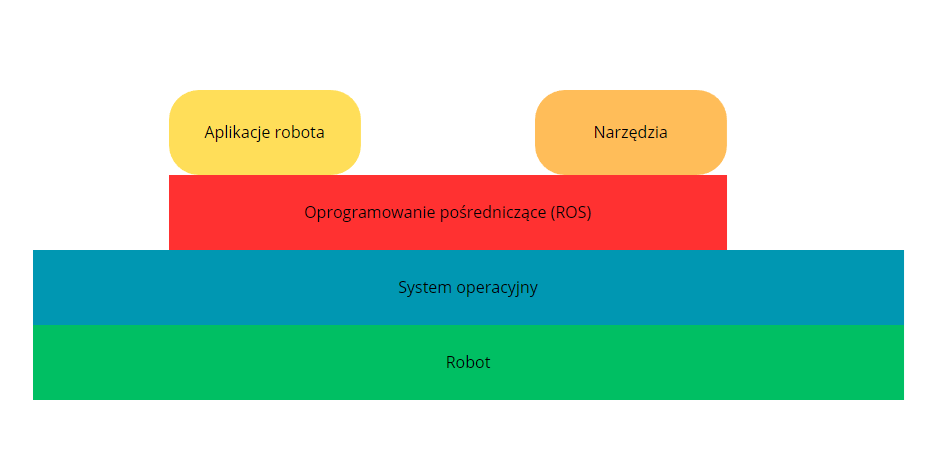
\includegraphics[width=0.8\textwidth]{images/middle.png}
	\caption{Reprezentacja pośrednika w systemie robota \cite{bib:ros2Concise}}
	\label{fig:middle}
	\end{figure}
\newline
Zasadniczo ROS 2 to otwartoźródłowe oprogramowanie bazujące na usłudze dystrybucji danych - DDS (ang. "Data Distribution Service"), które dostarcza ustandaryzowane narzędzia do organizacji kodu aplikacji w modularne pakiety, zapewniania współbieżnego wykonania kodu na wiele dostępnych plików wykonywalnych, oraz komunikację między tymi modułami podczas równoległego uruchomienia w systemie robota.\cite{bib:guide}

\newpage
\subsection{SLAM Toolbox}
SLAM Toolbox to zestaw narzędzi i rozwiązań do tworzenia map 2D w czasie rzeczywistym, stworzone przez Steve'a Mecenski.
 Stosowane algorytmy w przeszłości to np. GMapping, Karto, Cartographer oraz Hector, jednakże prawie żaden z nich nie potrafił tworzyć map w czasie rzeczywistym, jedynie Cartographer stworzony przez Google miał takie możliwości, lecz przestał być on wspierany.
 \cite{bib:slamtoolbox} Zastosowanie SLAM Toolbox pozwala na tworzenie map w czasie rzeczywistym obszarów, do nawet 24 000 m$^2$ przez niewykwalifikowanych użytkowników. Przykład działania SLAM Toolbox przedstawiono na rysunku poniżej.

\begin{figure}[h]
	\centering
	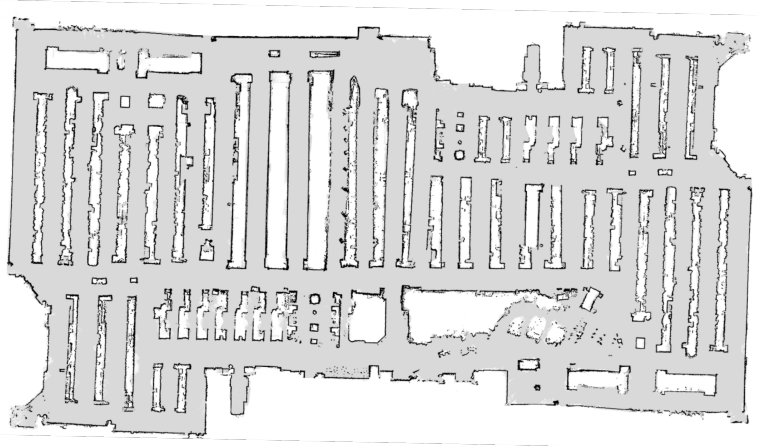
\includegraphics[width=0.8\textwidth]{images/sklep.png}
	\caption{Mapa dwóch pomieszczeń utworzona za pomocą SLAM Toolbox \cite{bib:slamtoolbox}}
	\label{fig:sklep}
	\end{figure}
\newpage
SLAM Toolbox oferuje 3 główne tryby pracy:
\begin{itemize}
	\item \textbf{Mapowanie synchroniczne} - Ten tryb pozwala na mapowanie i lokalizację w przestrzeni zachowując dane poprzednich pomiarów. Pozwala to na większą dokładność mapy kosztem szybkości i odporności na przerwania.
	\item \textbf{Mapowanie asynchroniczne} - W tym trybie mapowanie i lokalizacja odbywają się wyłącznie na podstawie aktualnych pomiarów gdy ostatnie pomiary zakończą się i zostanie spełnione kryterium dokładności. Pozwala to na szybsze i mniej podatne na przerwania mapowanie kosztem jakości.
	\item \textbf{Lokalizacja} - W tym trybie robot dopasowuje aktualne pomiary do istniejącej mapy w celu określenia swojej pozycji. System tworzy tymczasowe punkty odniesienia z nowych pomiarów, które są używane do precyzyjnej lokalizacji. Po określonym czasie te tymczasowe punkty są usuwane, przywracając oryginalną mapę. Tryb ten może również działać bez wcześniejszej mapy, wykorzystując tylko lokalne pomiary do nawigacji.
\end{itemize}

\newpage
\subsection{Navigation2 (Nav2) i lokalizacja}
Nav2 jest to pakiet narzędzi do nawigacji robotów mobilnych w ROS 2. Zawiera on zestaw algorytmów do tworzenia modeli środowiska z sensorów, dynamicznego planowania ścieżki, obliczania prędkości silników i omijania przeszkód. 
Pakiet wykorzystuje drzewa zachowań (ang. "Behavior Trees") do definiowania zachowań robota, przez implementację wielu niezależnych zadań. Niektóre z nich odpowiadają za np. obliczanie trasy do celu, inne za naprawę błędów, a jeszcze inne za omijanie przeszkód. Dzięki komunikacji między tymi zadaniami, robot jest w stanie wykonywać skomplikowane zadania nawigacyjne.
\cite{bib:abs-2003-00368}
\newline
\newline
Do lokalizacji robota na mapie można wykorzystać wcześniej opisany SLAM Toolbox, jednak w pakiecie Nav2 dostępny jest również pakiet AMCL (ang. "Adaptive Monte Carlo Localization")\cite{bib:amcl}, który pozwala na lokalizację robota na mapie z wykorzystaniem filtru cząsteczkowego. Algorytm ten polega na generowaniu losowych próbek (cząsteczek) reprezentujących możliwe położenia robota, a następnie porównywaniu ich z pomiarami z czujników. Cząsteczki, które najlepiej pasują do pomiarów są wybierane, a reszta jest odrzucana. W ten sposób algorytm estymuje pozycję robota na mapie. \cite{bib:amcl}
\subsection{ROS2 Control i sterowanie napędami}
ROS2 Control to platforma do sterowania, zarządzania i komunikacji pomiędzy urządzeniami w robotach z oprogramowaniem. \cite{bib:ros2control}. Rozwiazanie to umożliwia w łatwy sposób zarządzanie silnikami, enkoderami, czy innymi urządzeniami w robocie. Dzięki zastosowaniu ROS2 Control można wykorzystać np. pakiet diffdrive\_arduino, do sterowania robotem z napędem różnicowym za pomocą Arduino. Pakiet ten pozwala również na sterowanie prędkością silników, odczyt enkoderów, obliczanie odometrii oraz transformację między układem odometrii a układem bazowym. \cite{bib:diffdrive}
 

\section{Wybór rozwiązań}
Na podstawie analizy dostępnych narzędzi, w projekcie zdecydowano się na wykorzystanie SLAM Toolbox do mapowania, AMCL do lokalizacji podczas nawigacji, Nav2 do planowania ścieżki i kontroli ruchu oraz ROS2 Control z DiffDrive Arduino do sterowania napędami. Wybór ten podyktowany jest stabilnością rozwiązań, oraz dobrą integracją komponentów w ekosystemie ROS 2 oraz aktywnym wsparciem społeczności i dostępnością dokumentacji.


%\begin{Definition}\label{def:1}
%Definicja to zdanie (lub układ zdań) odpowiadające na pytanie o strukturze „co to jest a?”. Definicja normalna jest zdaniem złożonym z 2 członów: definiowanego (łac. definiendum) i definiującego (łac. definiens), połączonych spójnikiem definicyjnym („jest to”, „to tyle, co” itp.). 
%\end{Definition}
%
%\begin{Theorem}[Pitagorasa]\label{t:pitagoras}
%W dowolnym trójkącie prostokątnym suma kwadratów długości przyprostokątnych jest równa kwadratowi długości przeciwprostokątnej tego trójkąta. 
%\end{Theorem}
%
%\begin{Example}[generalizacja]\label{ex:generalizacja}
%Przykładem generalizacji jest para: zwierzę i pies. Pies jest zwierzęciem. Pies jest uszczegółowieniem pojęcia zwierzę. Zwierzę jest uogólnieniem pojęcia pies.
%\end{Example}

%%%%%%%%%%%%%%%%%%%%%%%%




% TODO
\chapter{Wymagania i narzędzia}
\label{ch:wymagania-i-narzedzia}

W niniejszym rozdziale przedstawiono wymagania funkcjonalne systemu, przypadki użycia w formie diagramu UML, szczegółową specyfikację wykorzystanych komponentów sprzętowych oraz metodykę i etapy realizacji projektu.

\section{Wymagania funkcjonalne}
System powinien realizować następujące funkcje:
\begin{itemize}
\item Zdalne sterowanie robotem poprzez klawiaturę (teleop\_twist\_keyboard \cite{bib:teleop}) w celu eksploracji i mapowania otoczenia
\item Tworzenie i zapisywanie mapy otoczenia w czasie rzeczywistym 
\item Lokalizacja robota na zapisanej mapie z wykorzystaniem algorytmu AMCL
\item Autonomiczna nawigacja do wyznaczonych punktów na mapie z omijaniem przeszkód

\end{itemize}
\newpage
\section{Przypadki użycia}
Na rysunku \ref{fig:use-case} przedstawiono diagram przypadków użycia systemu. System umożliwia użytkownikowi zdalne sterowanie robotem, tworzenie mapy otoczenia, lokalizację robota na mapie oraz autonomiczną nawigację do wyznaczonych punktów. 
\begin{figure}[!hb]
\centering
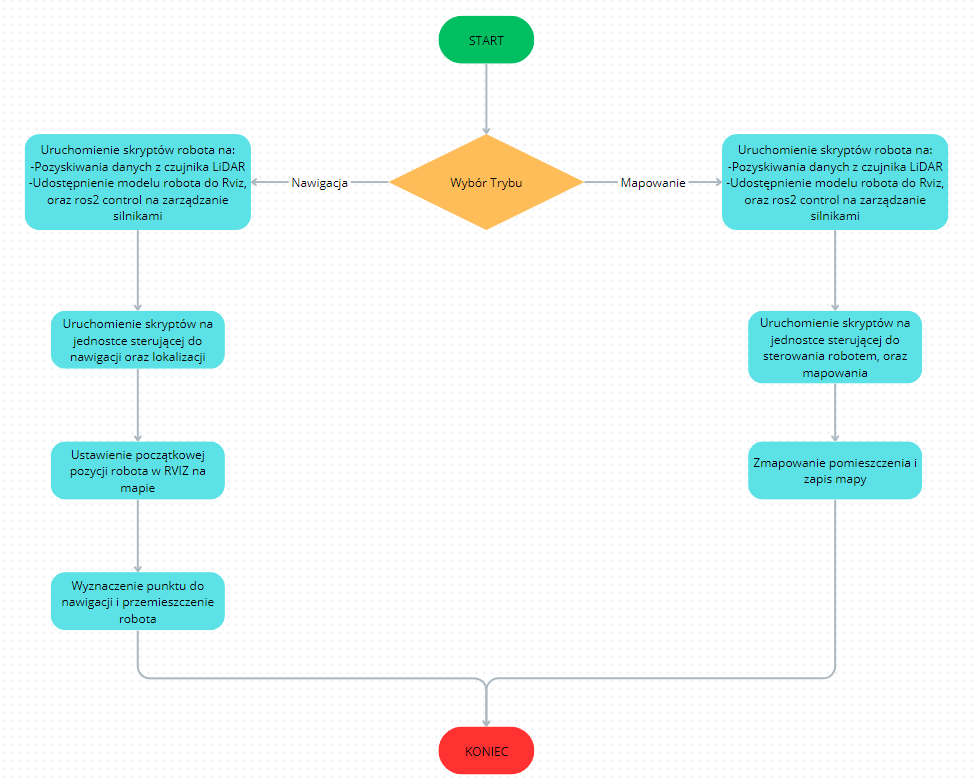
\includegraphics[width=0.8\textwidth]{images/UML.png}
\caption{Diagram przypadków użycia systemu}
\label{fig:use-case}
\end{figure}
\newpage
\section{Specyfikacja komponentów}
\subsection{Jednostki sterujące}
\begin{itemize}
\item Raspberry Pi 4 - główny komputer zarządzający robotem:
	\begin{itemize}
	\item System operacyjny Ubuntu 22.04
	\item ROS 2 Humble
	\item Komunikacja przez SSH z jednostką sterującą zachowaniem robota
	\end{itemize}
	
		
\item Arduino Nano - sterownik silników:
	\begin{itemize}
	\item Obsługa enkoderów
	\item Komunikacja szeregowa z Raspberry Pi
	\end{itemize}


\end{itemize}

\subsection{Napęd}
\begin{itemize}
\item 2x silnik DC 12V 240RPM z metalową przekładnią
\item Wbudowane enkodery magnetyczne Halla


\item Sterownik L298N - dwukanałowy mostek H \newline

\end{itemize}


\subsection{Zasilanie}
\begin{itemize}
\item 6x akumulatory Li-ion 18650:
	\begin{itemize}
	\item 4 ogniwa (2S2P) dla silników
	\item 2 ogniwa (2S) dla elektroniki
	\end{itemize}
	

\item 2x przetwornica step-down:
	\begin{itemize}
	\item 12V dla silników
	\item 5V dla Raspberry Pi
	\end{itemize}

		\newpage
\end{itemize}



\section{Budowa robota i sposób połączenia silników z kontrolerem}


\begin{figure}[!hb]
	\centering
	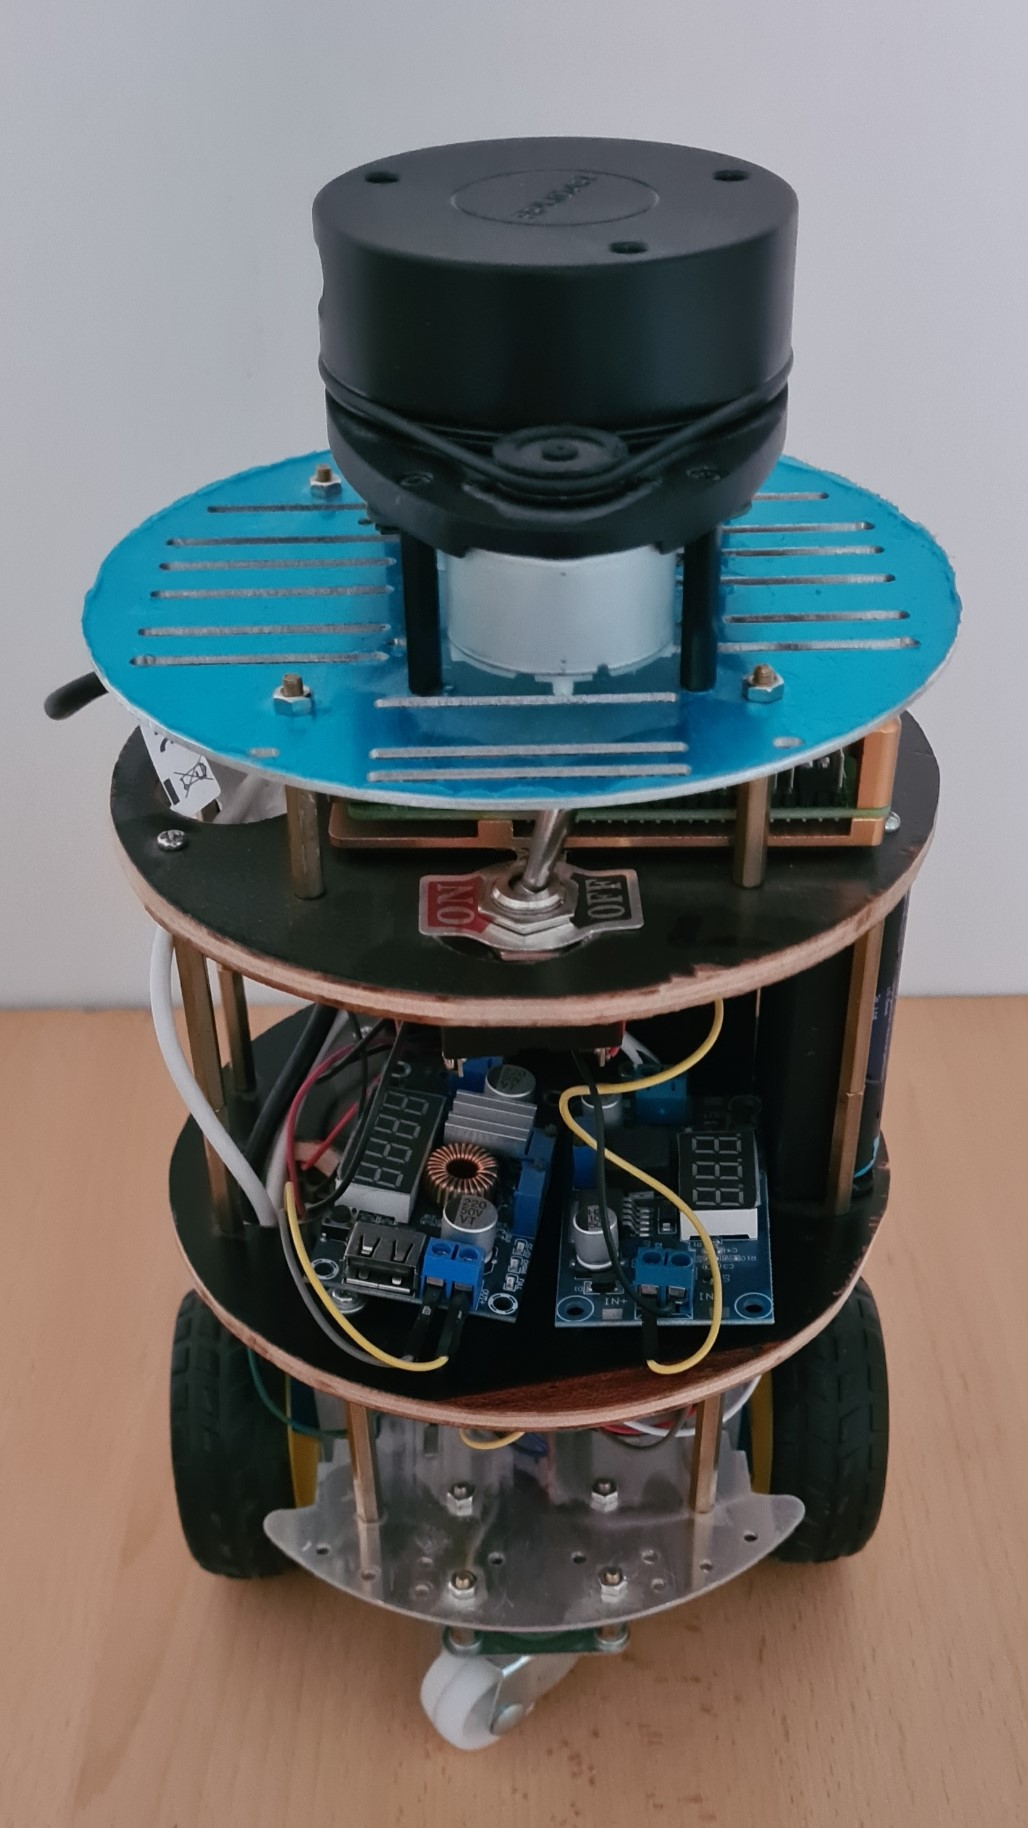
\includegraphics[width=0.7\textwidth]{images/robot.jpg}
	\caption{Zdjęcie przedstawiające zbudowanego robota}
	\label{fig:robot-zdj}
	\end{figure}
	\newpage

	\begin{figure}[!hb]
		\centering
		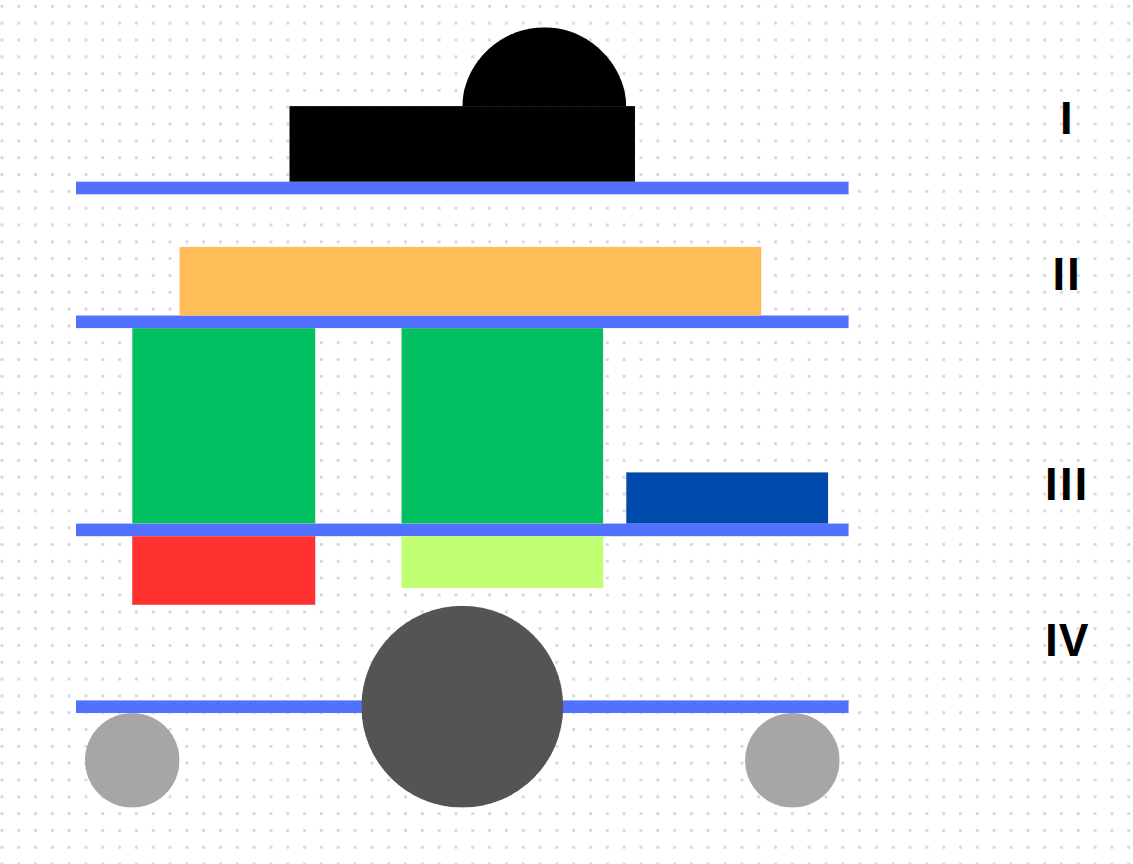
\includegraphics[width=0.7\textwidth]{images/schemat-robot.png}
		\caption{Uproszczony schemat przedstawiający budowę robota}
		\label{fig:robot-schemat}
		\end{figure}
Na schemacie z rysunku \ref{fig:robot-schemat} przedstawiono konkretne poziomy robota, takie jak:
\begin{itemize}
	\item Poziom I - LiDAR RPLidar A1 (Czarny element)
	\item Poziom II - Raspberry Pi 4 (Pomarańczowy element)
	\item Poziom III - Akumulatory (Zielone elementy) i przetwornice (Niebieski element)
	\item Poziom IV - Arduino Nano (Żółty element) i sterownik L298N (Czerwony element) z silnikami (Szare elementy)
\end{itemize}
\newpage

\begin{figure}[!hb]
	\centering
	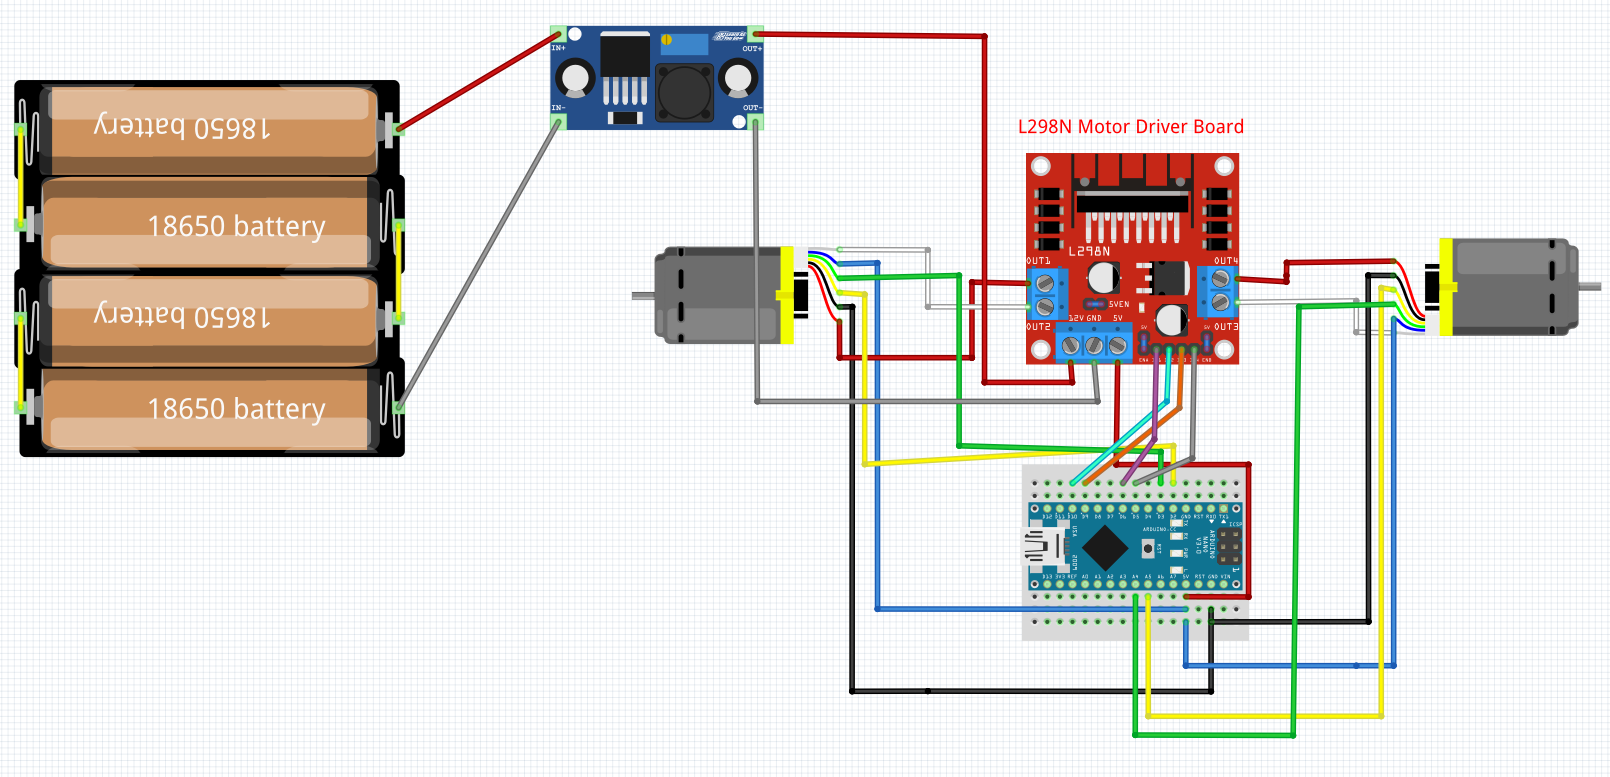
\includegraphics[width=1\textwidth]{images/schema_arduino.png}
	\caption{Schemat połączenia silników z Arduino i L298N}
	\label{fig:arduino-schema}
	\end{figure}
Na zaprezentowanym schemacie rys. \ref{fig:arduino-schema} przedstawiono sposób połączenia silników z Arduino i sterownikiem L298N. Silniki DC z enkoderami są zasilane z akumulatorów Li-ion, a sterowane przez Arduino Nano za pomocą sterownika L298N. Enkodery są podłączone do Arduino, które odczytuje impulsy i oblicza prędkość i położenie robota. Komunikacja między Arduino a Raspberry Pi odbywa się przez port szeregowy, co umożliwia przesyłanie danych o prędkości i położeniu robota.

\newpage
\begin{figure}[!hb]
	\centering
	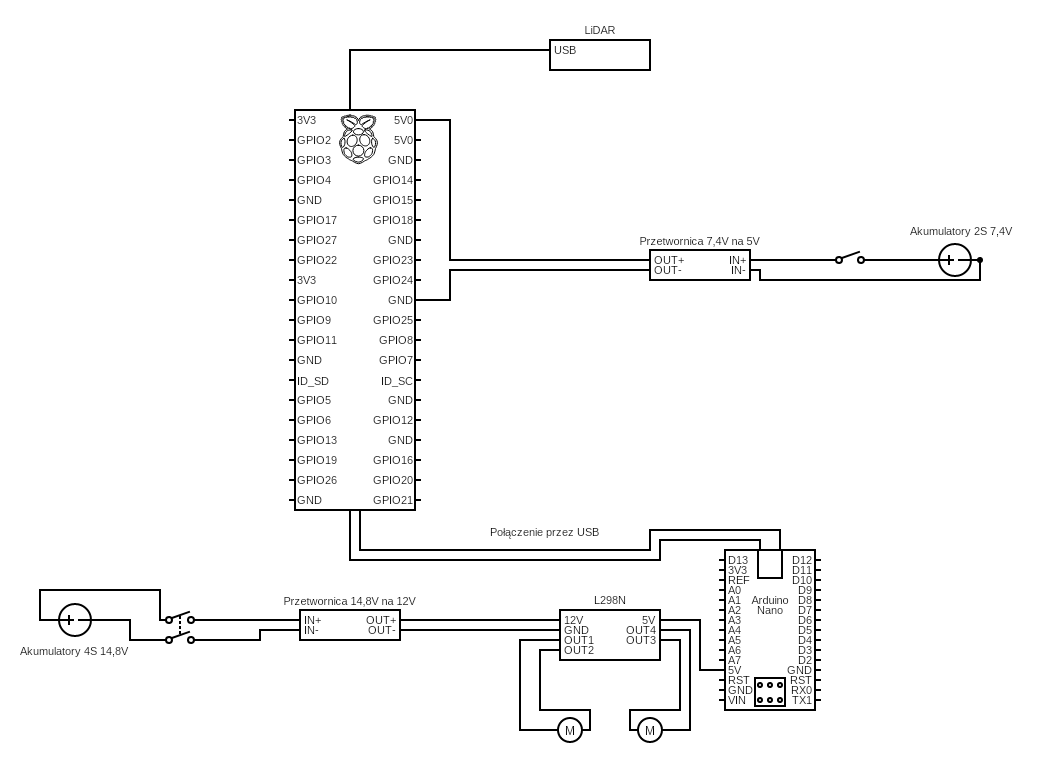
\includegraphics[width=0.8\textwidth]{images/circuit.png}
	\caption{Schemat elektryczny}
	\label{fig:schemat-elektryczny}
	\end{figure}
Na schemacie \ref{fig:schemat-elektryczny} przedstawiono sposób połączenia wszystkich komponentów elektrycznych w robocie. Akumulatory zasilają silniki i elektronikę, a przetwornice step-down dostarczają odpowiednie napięcia do poszczególnych komponentów. Sterownik L298N steruje silnikami, a Arduino Nano odczytuje enkodery i przesyła dane do Raspberry Pi. Raspberry Pi zarządza robotem, odbiera dane z czujników i steruje silnikami. 
\newpage

\section{Metodyka i etapy realizacji}
\subsection{Etap 1: Przygotowanie platformy sprzętowej}
\begin{itemize}
\item Instalacja systemu Ubuntu 22.04 na Raspberry Pi
\item Konfiguracja połączenia SSH
\item Instalacja ROS 2 Humble
\end{itemize}

\subsection{Etap 2: Implementacja sterowania napędem}
\begin{itemize}
\item Podłączenie silników do sterownika L298N
\item Programowanie Arduino - obsługa silników i enkoderów
\item Implementacja komunikacji szeregowej z Raspberry Pi
\end{itemize}

\subsection{Etap 3: Integracja sensorów}
\begin{itemize}
\item Montaż i konfiguracja LiDAR-a
\item Kalibracja czujników
\item Opracowanie układu mechanicznego i obudowy
\end{itemize}

\subsection{Etap 4: Implementacja oprogramowania}
\begin{itemize}
\item Konfiguracja pakietów ROS 2:
	\begin{itemize}
	\item SLAM Toolbox do mapowania
	\item Nav2 do nawigacji z AMCL do lokalizacji
	\item ROS2 Control do sterowania napędem
	\end{itemize}
\item Integracja i testy systemu
\end{itemize}



% TODO
\chapter{Specyfikacja użytkowa}
\label{ch:04}
W tym rozdziale przedstawiono wymagania użytkownika oraz specyfikację funkcjonalną systemu. Opisano kategorie użytkowników, sposób obsługi, administrację systemem, kwestie bezpieczeństwa oraz przykłady działania systemu.


\subsection{Wymagania sprzętowe i programowe}
Projekt ten stworzony był z myślą o następujących wymaganiach dla robota:
\newline\newline
Sprzętowe:
\begin{itemize}
	\item Poruszać się w przestrzeni za pomocą sinlików, czyli np. przemieszczanie się do przodu, do tyłu, skręcanie w lewo i w prawo po korytarzach, czy w pomieszczeniach z równym podłożem.
	\item Skanować pomieszczenia za pomocą LiDAR-a, czyli zbieranie danych o otoczeniu wokół robota.
	\end{itemize}
Programowe:
\begin{itemize}
	\item Tworzyć mapę otoczenia, czyli zapisywanie danych z LiDAR-a w formie mapy 2D w czasie rzeczywistym i wizualizację tych danych w programie Rviz.
	\item Lokalizować się na mapie, czyli określanie pozycji robota na zapisanej mapie.
	\item Nawigować do wyznaczonych punktów, czyli planowanie trasy do punktów na mapie i omijanie przeszkód.
\end{itemize}
\newpage

\subsection{Sposób aktywacji i korzystania z robota z przykadem działania}
Sekcja ta zawiera szczegółowy opis korzystania z robota, od uruchomienia, sterowanie, mapowanie, zapis mapy, lokalizację i nawigację.

Pierwszym krokiem jest uruchomienie robota, w tym celu należy włączyć zasilanie dla Raspberry Pi i silników.


Następnie należy przygotować terminale na jednostce sterującej (dwa terminale mają być połączone przez protokuł ssh z Raspberry Pi, a cztery terminale mają być przygotowane na samej jednostce sterującej do uruchomienia późniejszych skryptów ROS). Przygotowanie tych terminali polega na odpowiednim:
\newline
Dla jednostki sterującej: wejsciu do katalogu roboczego, uruchomienie komend source /opt/ros/humble/setup.bash, oraz source /install/setup.bash.
\newline\newline
Dla Raspberry Pi: wejsciu do katalogu roboczego, uruchomienie komend source /opt/ros/humble/setup.bash, oraz source /install/setup.bash.
\newline\newline
Następnie, należy uruchomić 2 skrypty na Raspberry Pi, które odpowiadają za uruchomienie odpowiednich węzłów ROS. Pierwszy skrypt odpowiada za uruchomienie węzła odpowiedzialnego za sterowanie silnikami i udostępnienie modelu robota do RVIZ, a drugi za uruchomienie węzła odpowiedzialnego za odczyt danych z LiDAR-a. Odpowiednie komendy to: ros2 launch robot\_slam model\_controll.launch.py oraz ros2 launch robot\_slam rplidar.launch.py.
\newline\newline
\newpage
Po uruchomieniu tych skryptów, należy uruchomić program Rviz, który pozwala na wizualizację mapy i położenia robota. Komenda to: rviz2. Następnym krokiem jest uruchomienie skryptu odpowiedzialny za sterowanie robotem za pomocą klawiatury. Komenda to: ros2 launch robot\_teleop.launch.py. W tym momencie należy przejść do terminala na jednostce sterującej, i za pomocą klawiatury sterować robotem. 
\newline

Kolejnym krokiem jest uruchomienie skryptu odpowiedzialnego za mapowanie otoczenia. Komenda to: ros2 launch robot\_slam slam.launch.py. W tym momencie gdy robot przemieszcza się przez komendy z klawiatury, pomieszczenie jest mapowane.

\begin{figure}[!hb]
	\centering
	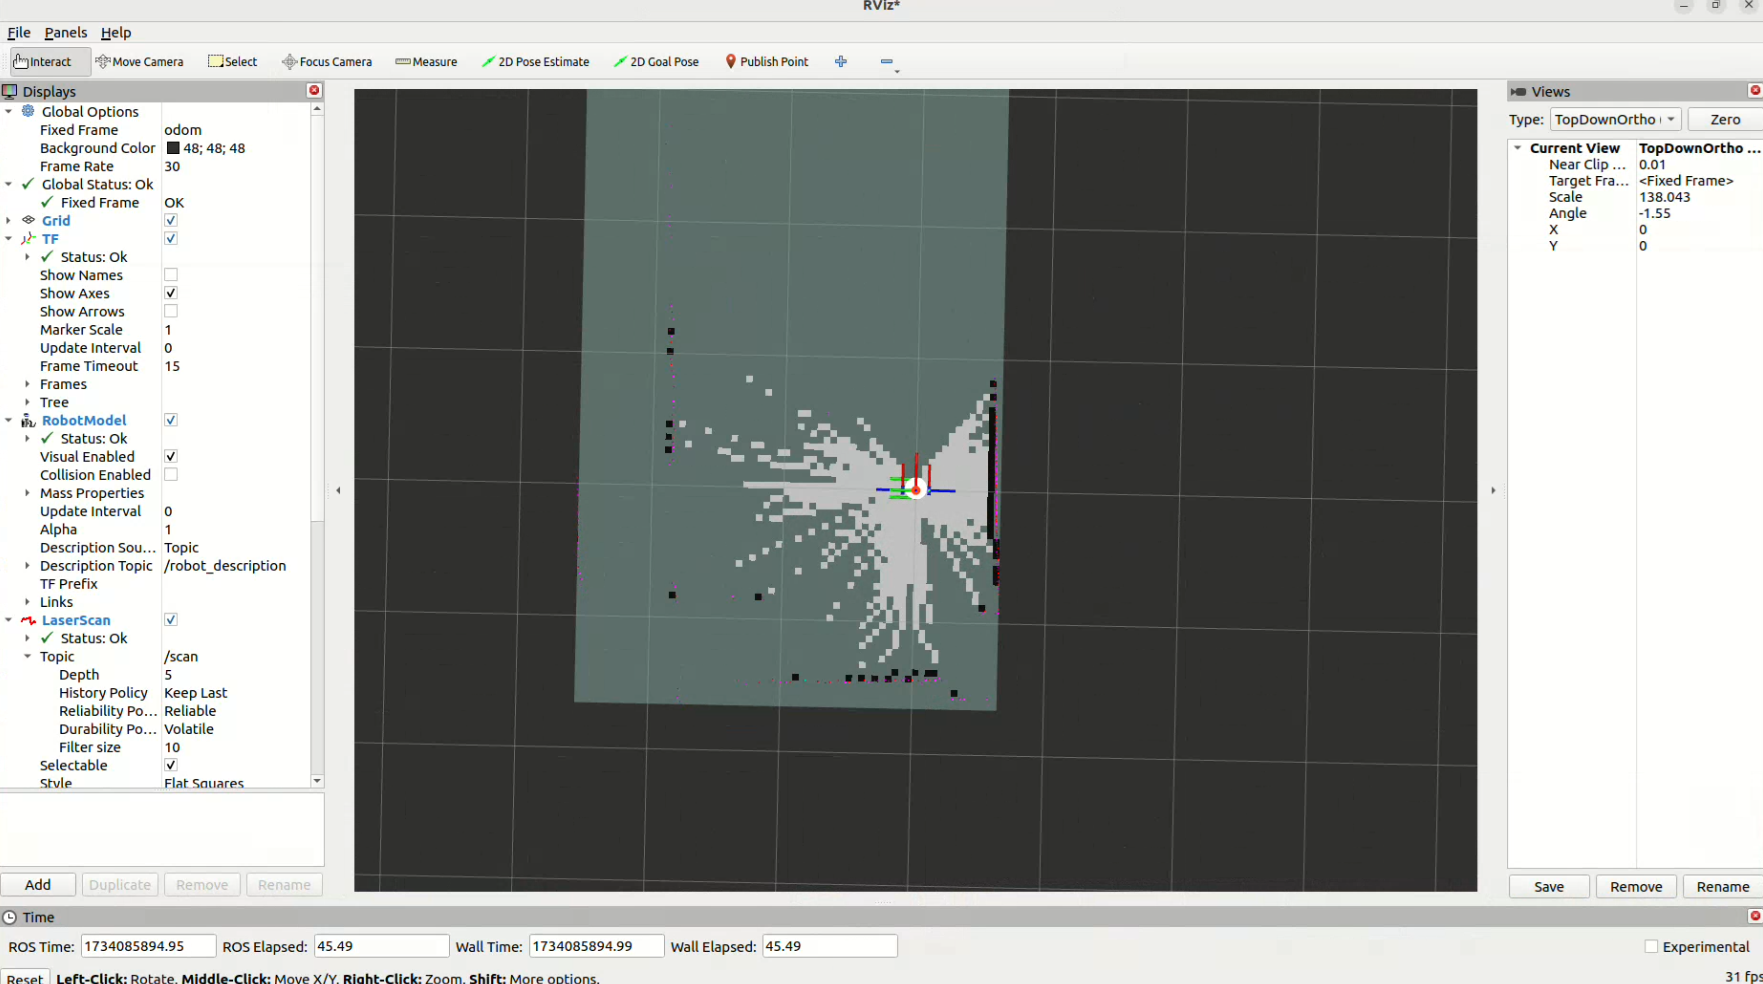
\includegraphics[width=1\textwidth]{images/launch-map.png}
	\caption{Okno RVIZ po uruchomieniu skryptów.}
	\label{fig:launch-map}
\end{figure}

\newpage
Gdy wystarczająco dużo pomieszczenia zostanie zmapowane, należy zapisać mapę. Można to wykonać przez komendę ros2 run nav2\_map\_server map\_saver -f map, lub przez dodanie panelu do RVIZ z zestawu narzędzi SLAM Toolbox i zapisanie mapy z poziomu tego panelu.

\begin{figure}[!hb]
	\centering
	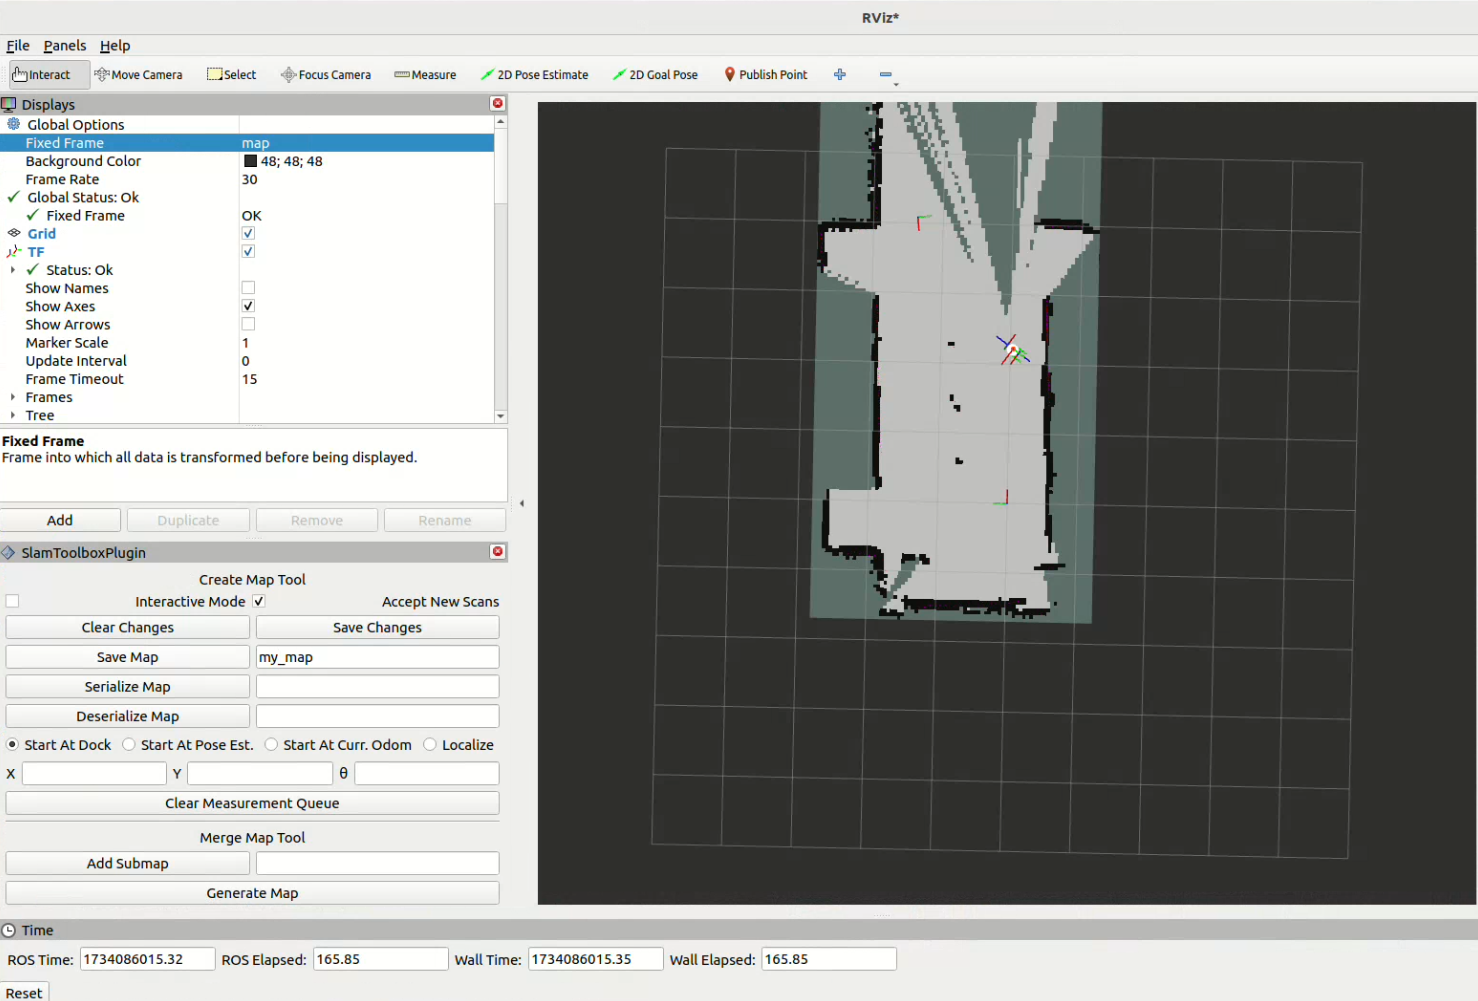
\includegraphics[width=1\textwidth]{images/save-map.png}
	\caption{Zmapowane pomieszczenie i zapis mapy jako plik my\_map.}
	\label{fig:save-map}
\end{figure}
\newpage
Z tak zapisaną mapą można zamknąć skrypty odpowiedzialne za sterowanie, mapowanie i RVIZ.
\newline\newline
Następnie, należy uruchomić skrypt odpowiedzialny za lokalizację robota na mapie, oraz nawigację robota.\newline Komenda to: ros2 launch robot\_slam nav\_localization.launch.py. 
W wyniku uruchomienia tego programu uruchomiony zostaje nowy ekran RVIZ z widoczną wcześniej zapisaną mapą.


Należy na niej umieścić robota przez wybranie z górnego zestawu narzędzi 2D Pose Estimate, a następnie kliknięcie na mapie w miejscu gdzie znajduje się robot, należy w tym momencie przez obrócenie w odpowiednim kierunku zielonej strzałki ustalić kierunek w jakim znajduje się robot,
 w wyniku czego algorytm AMCL tworzy chmurę przewidywanych punktów w których może znajdować się robot.
\begin{figure}[!hb]
	\centering
	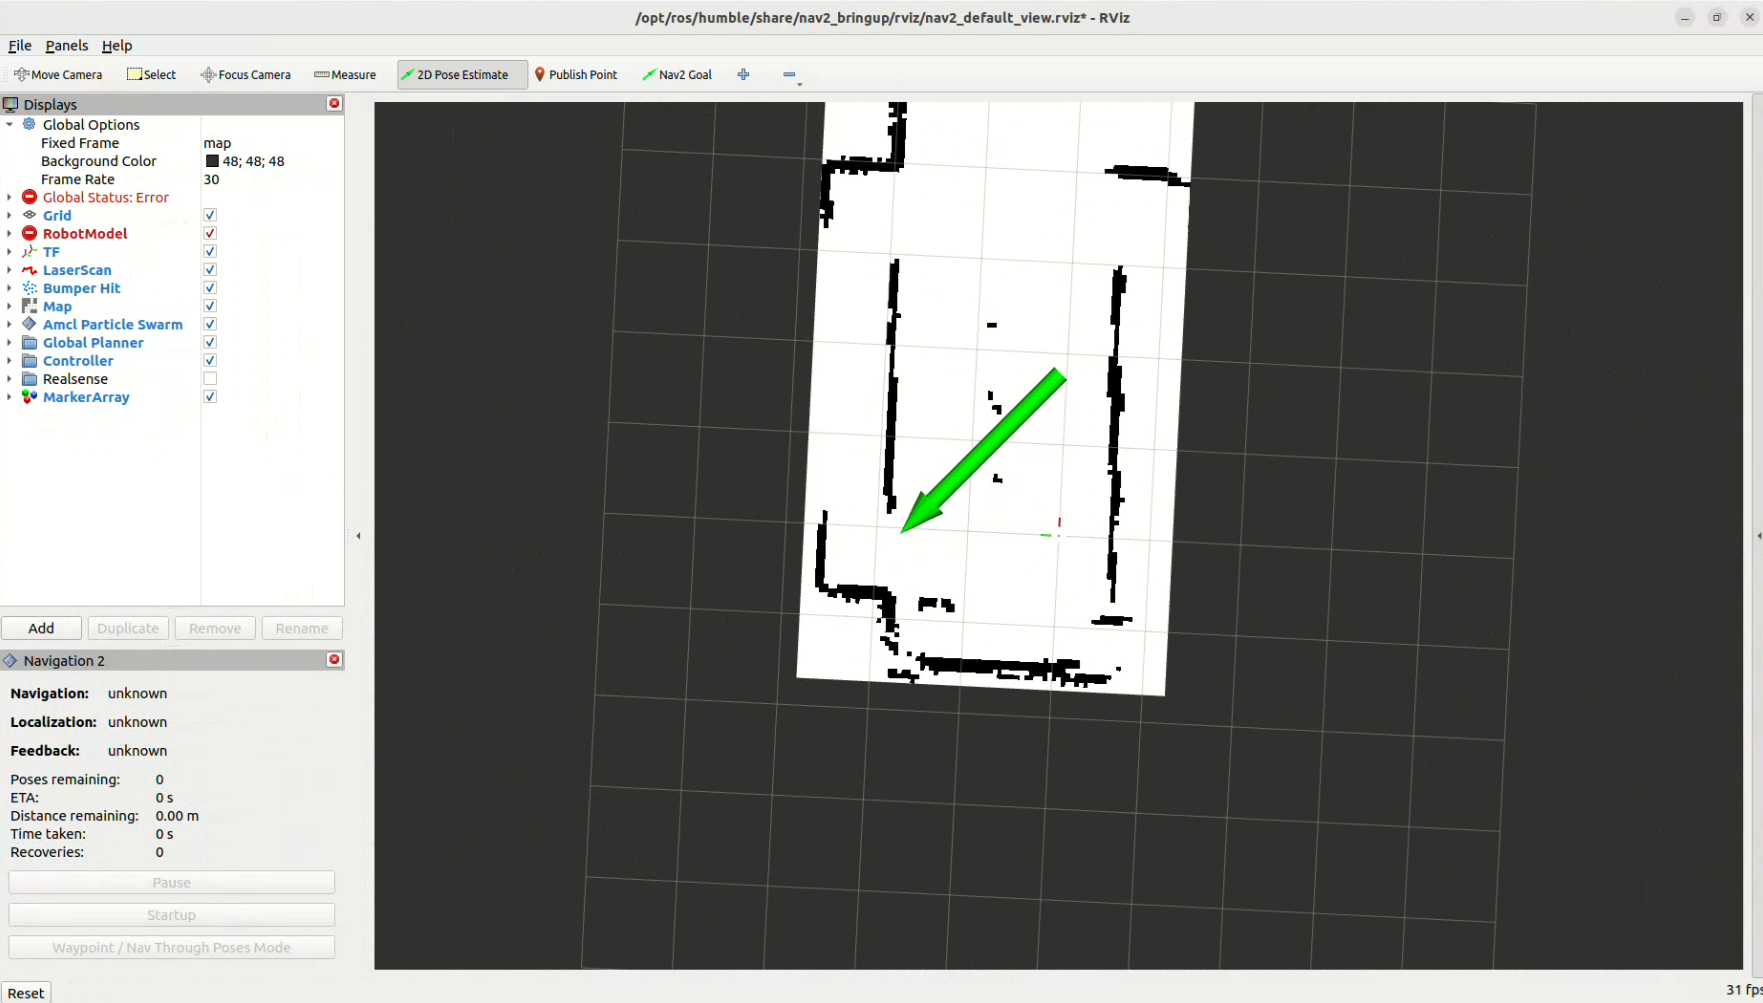
\includegraphics[width=1\textwidth]{images/launch-nav.png}
	\caption{RVIZ po uruchomieniu skryptu do lokalizacji i nawigacji i wybraniu pozycji robota.}
	\label{fig:nav-map}
\end{figure}
\newpage
\begin{figure}[!hb]
	\centering
	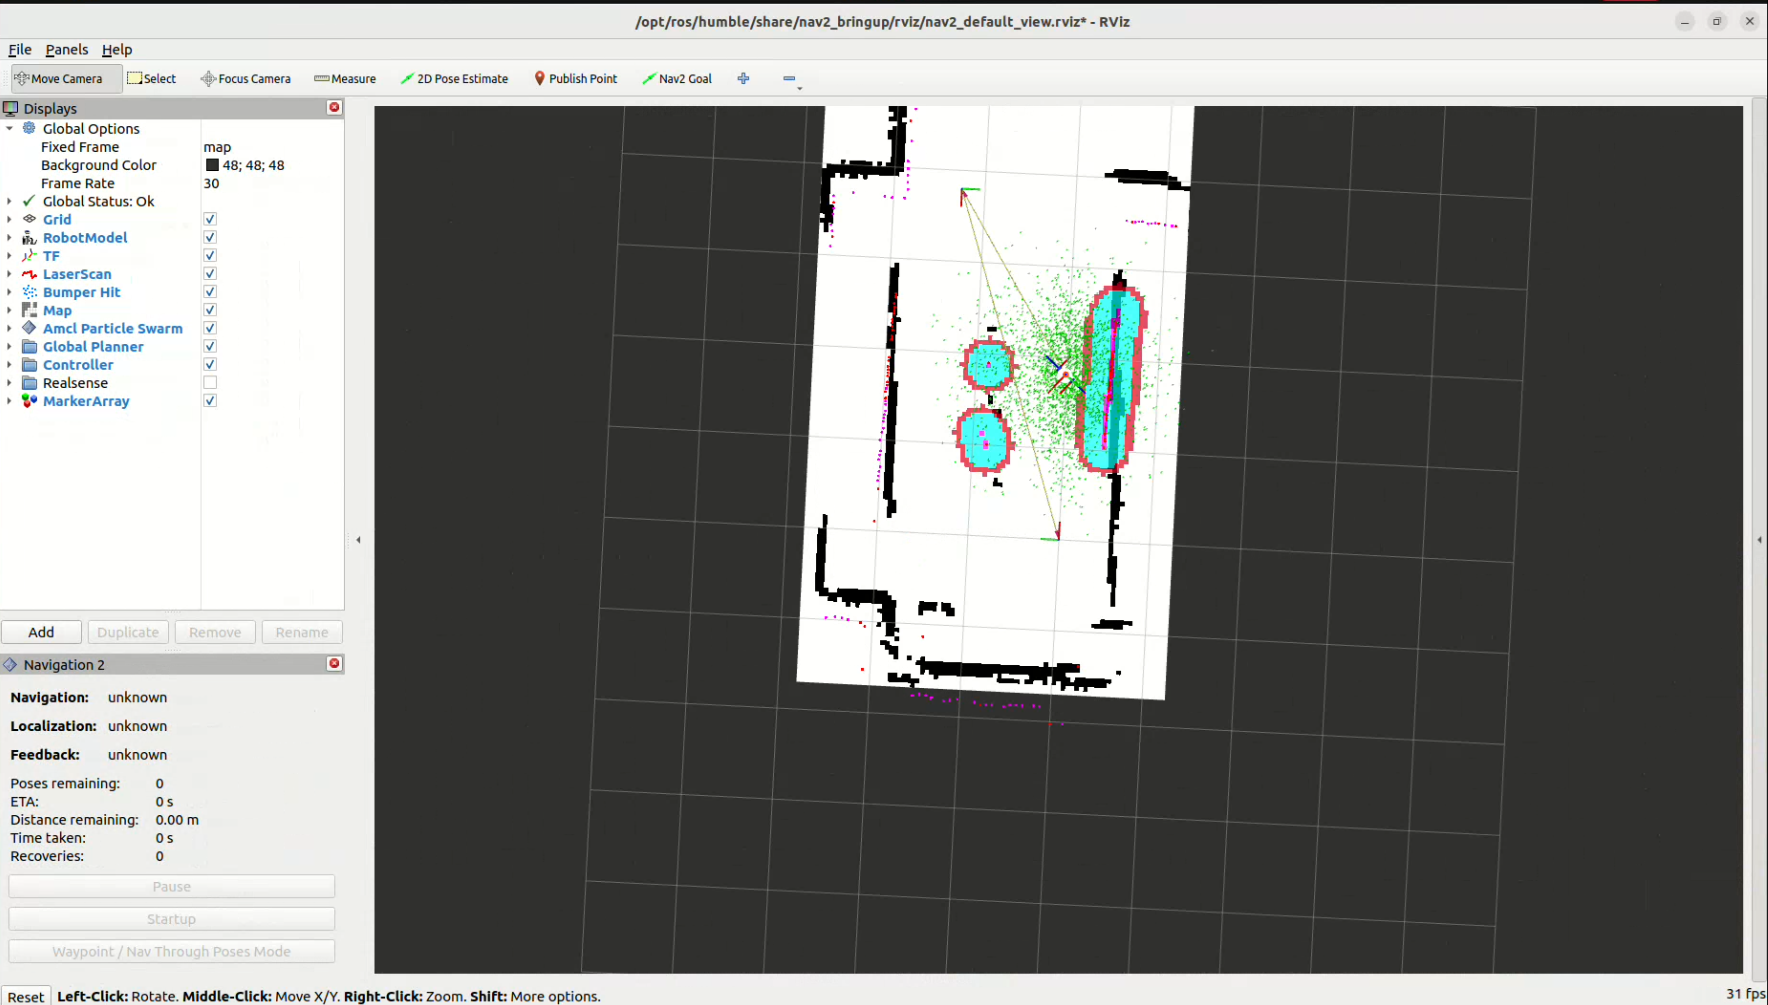
\includegraphics[width=1\textwidth]{images/launch-nav2.png}
	\caption{Wizualizacja rozproszonych punktów lokalizacji robota.}
	\label{fig:nav-map2}
\end{figure}
\newpage
Następnie należy wybrać cel do którego robot ma się przemieścić, przez wybranie z górnego zestawu narzędzi Nav2 Goal, a następnie kliknięcie na mapie w miejscu gdzie ma się znaleźć cel z ustawieniem zielonej strzałki w kierunku w jaki ma się ustawić.
\begin{figure}[!hb]
	\centering
	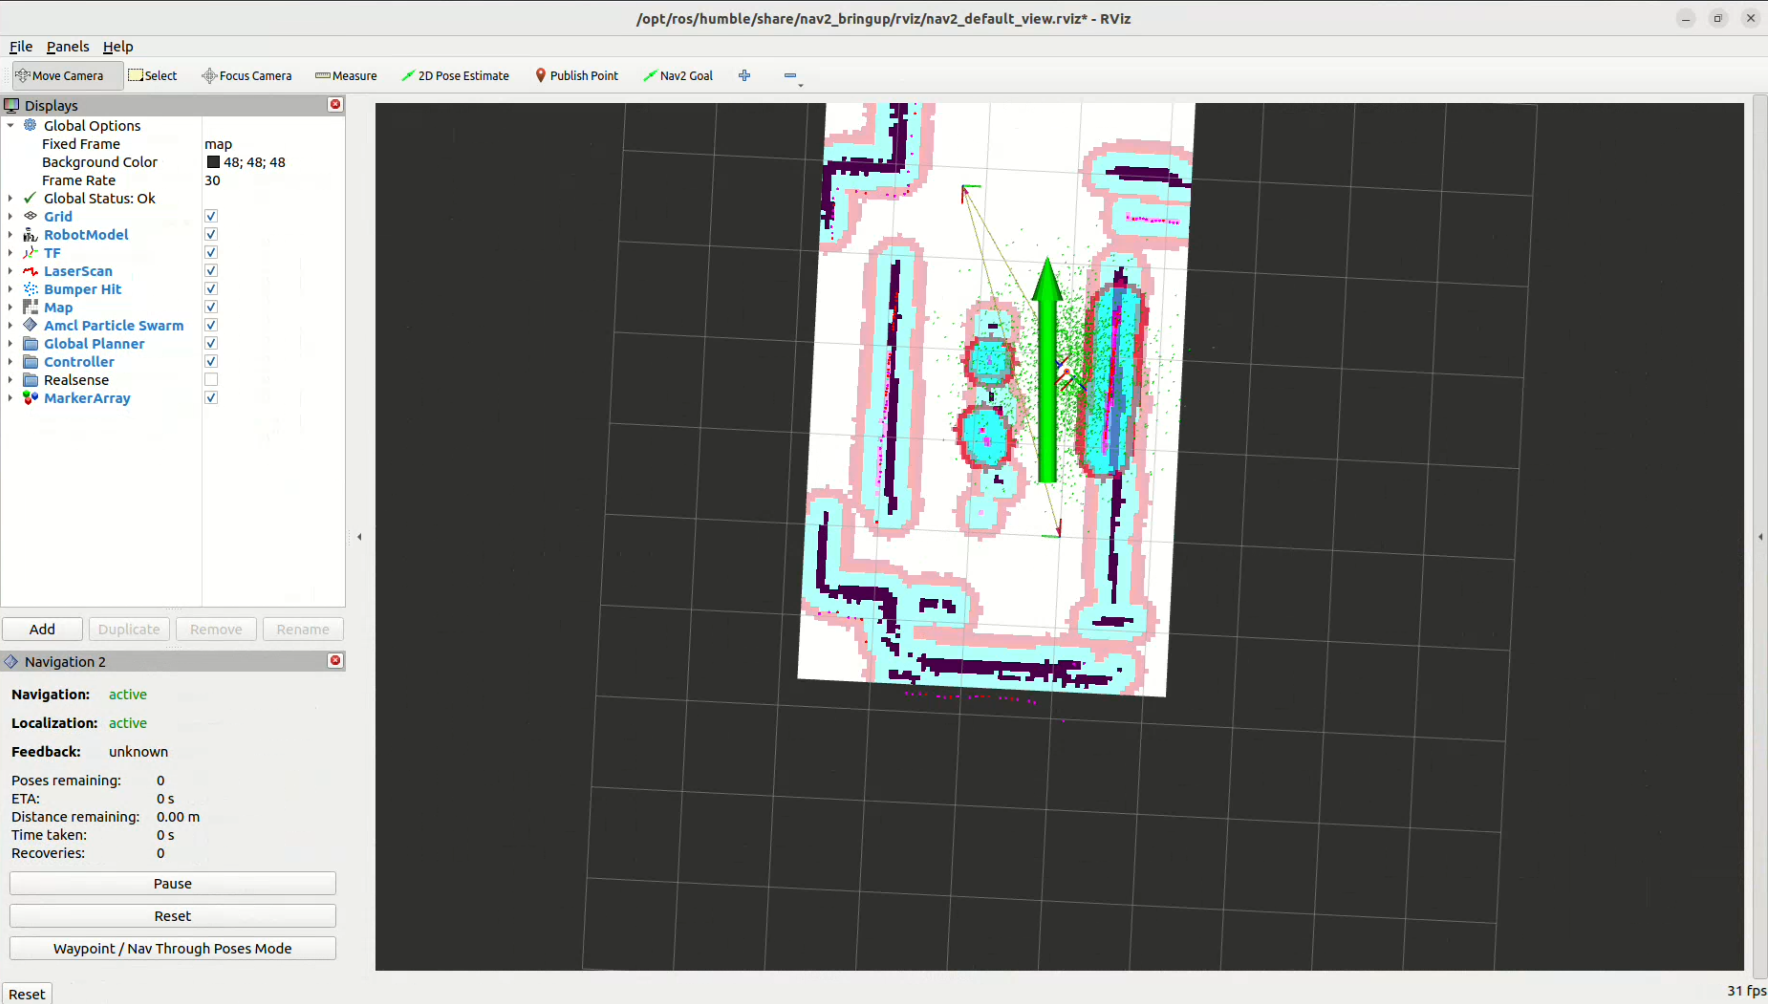
\includegraphics[width=1\textwidth]{images/launch-nav3.png}
	\caption{Wybór celu robota.}
	\label{fig:nav-map3}
\end{figure}
\newpage
Robot po wybraniu celu zaczyna poruszać się w kierunku celu, omijając przeszkody na swojej drodze.
\begin{figure}[!hb]
	\centering
	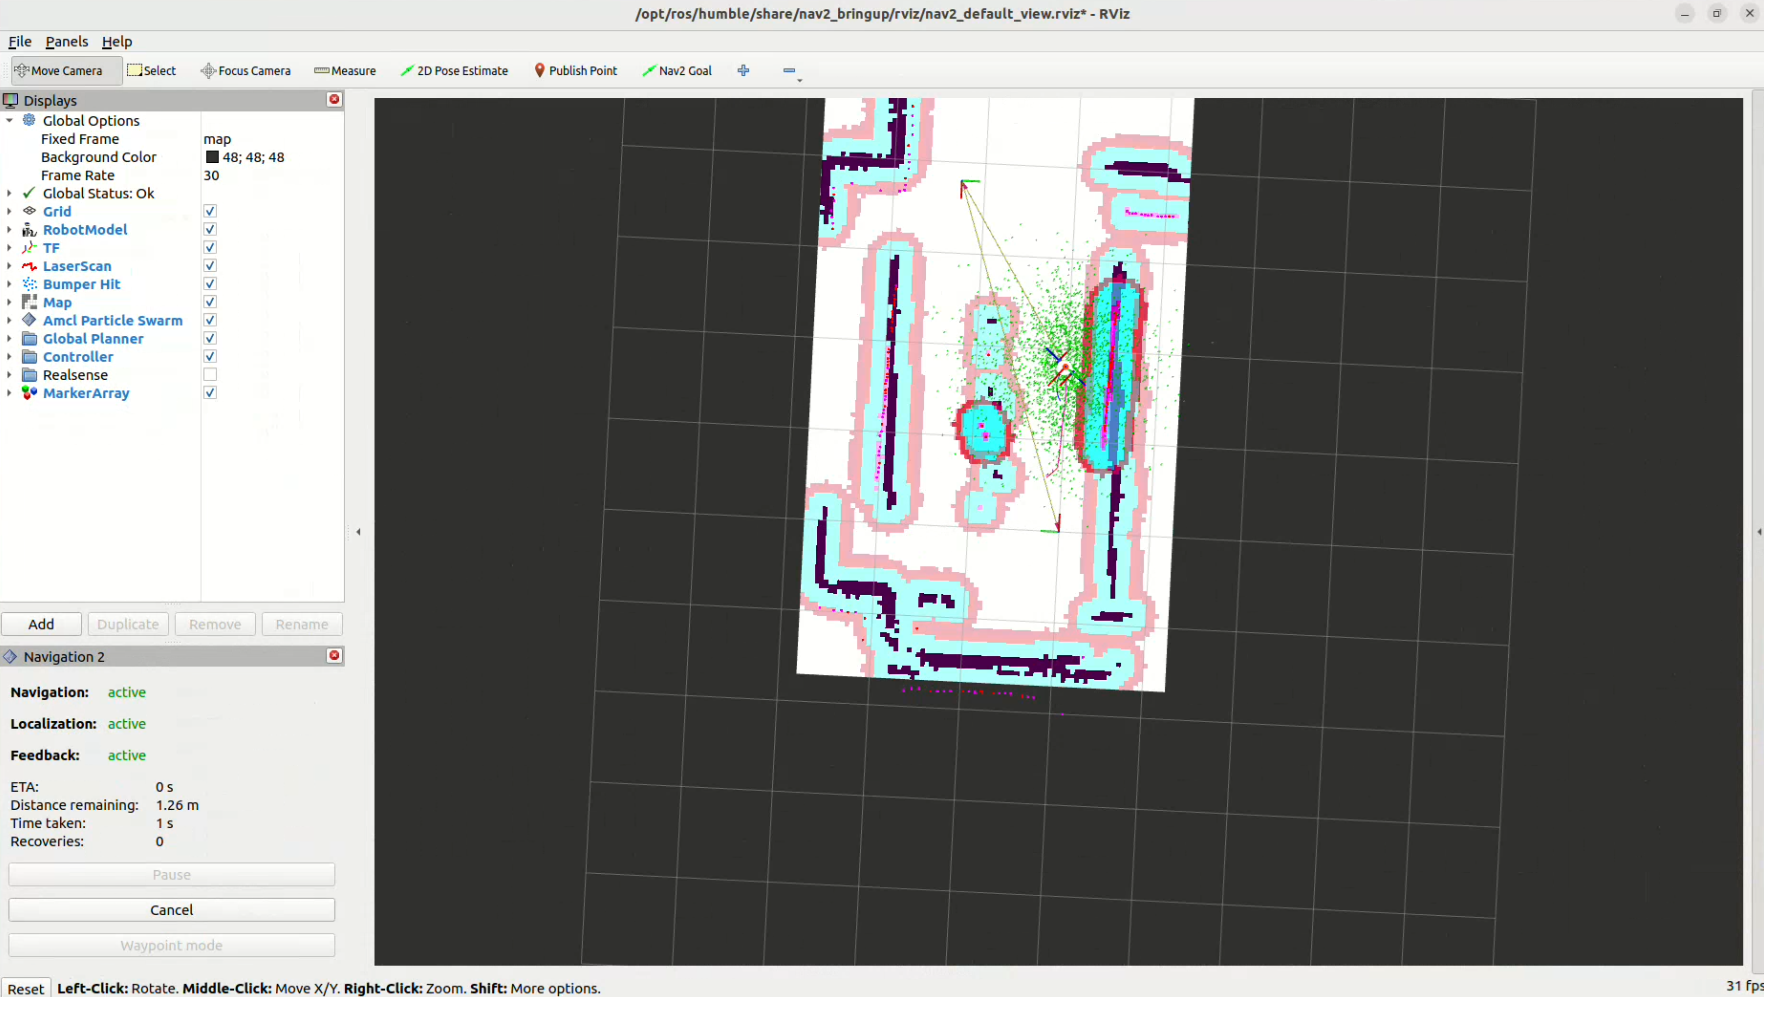
\includegraphics[width=1\textwidth]{images/launch-nav4.png}
	\caption{Wyznaczenie trasy.}
	\label{fig:nav-map4}
\end{figure}
\begin{figure}[!hb]
	\centering
	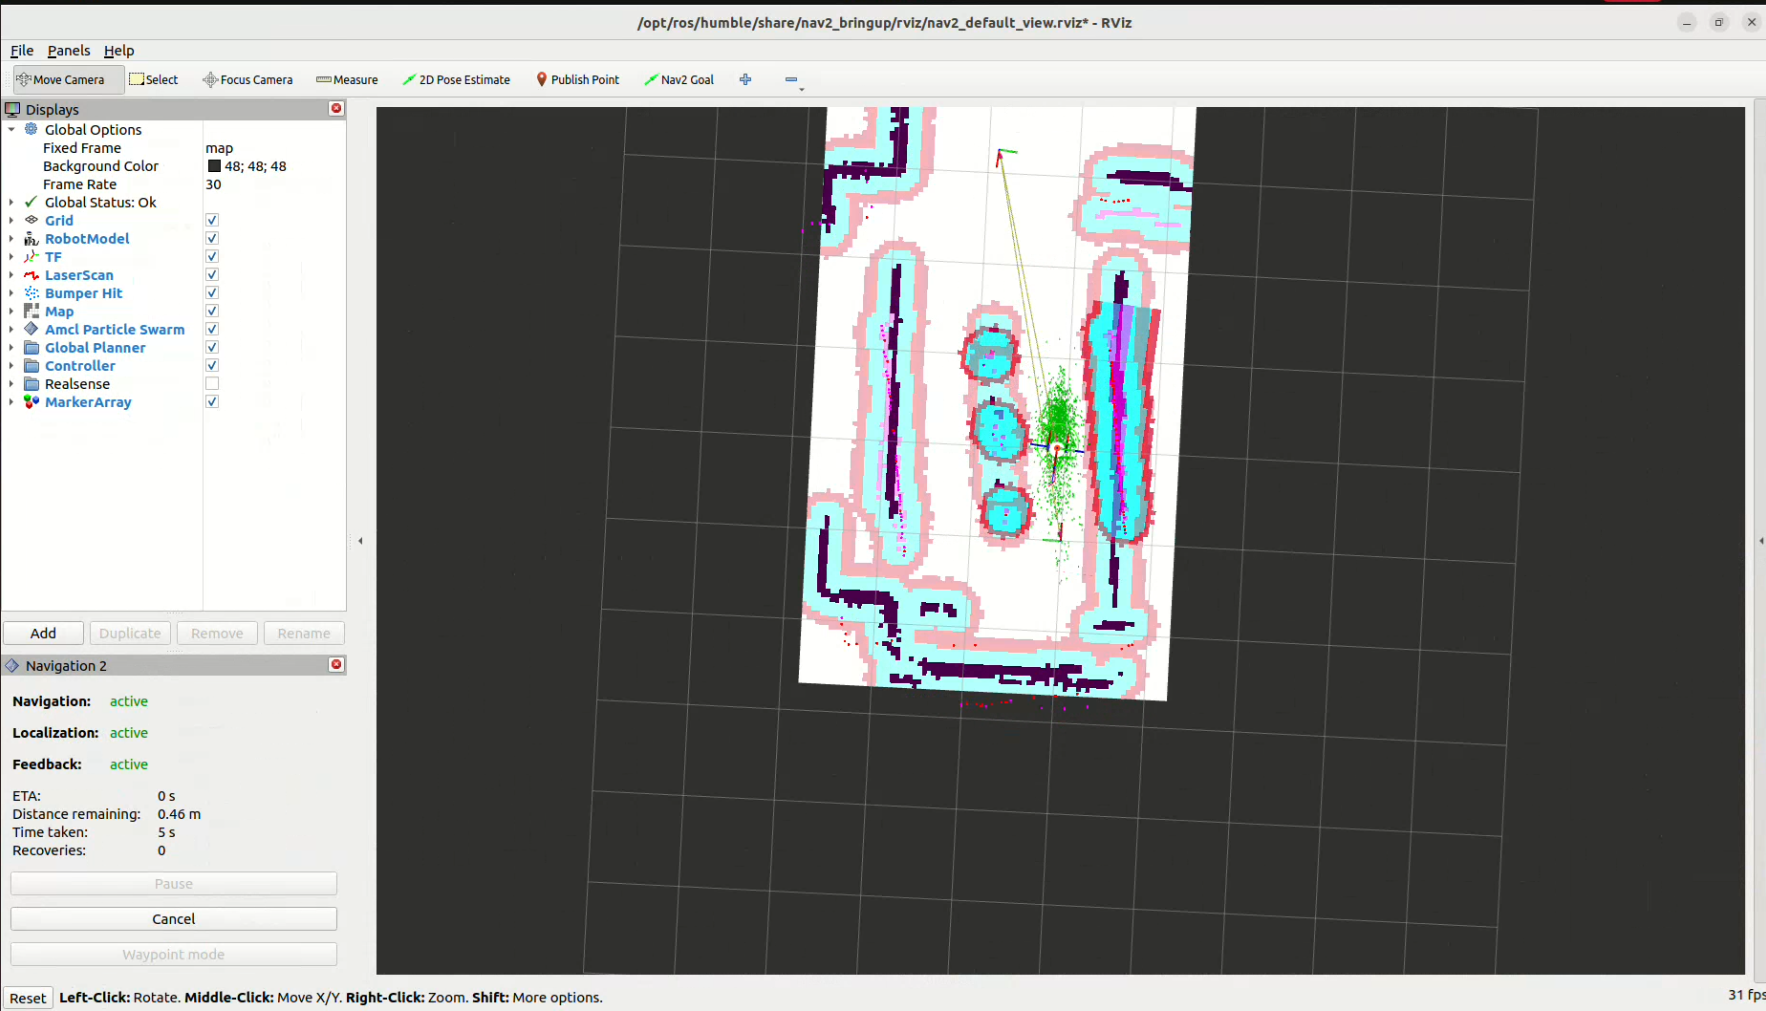
\includegraphics[width=1\textwidth]{images/launch-nav5.png}
	\caption{Nawigacja robota i zmniejszanie się chmury przewidywanej lokalizacji robota.}
	\label{fig:nav-map5}
\end{figure}
\newpage
\begin{figure}[!hb]
	\centering
	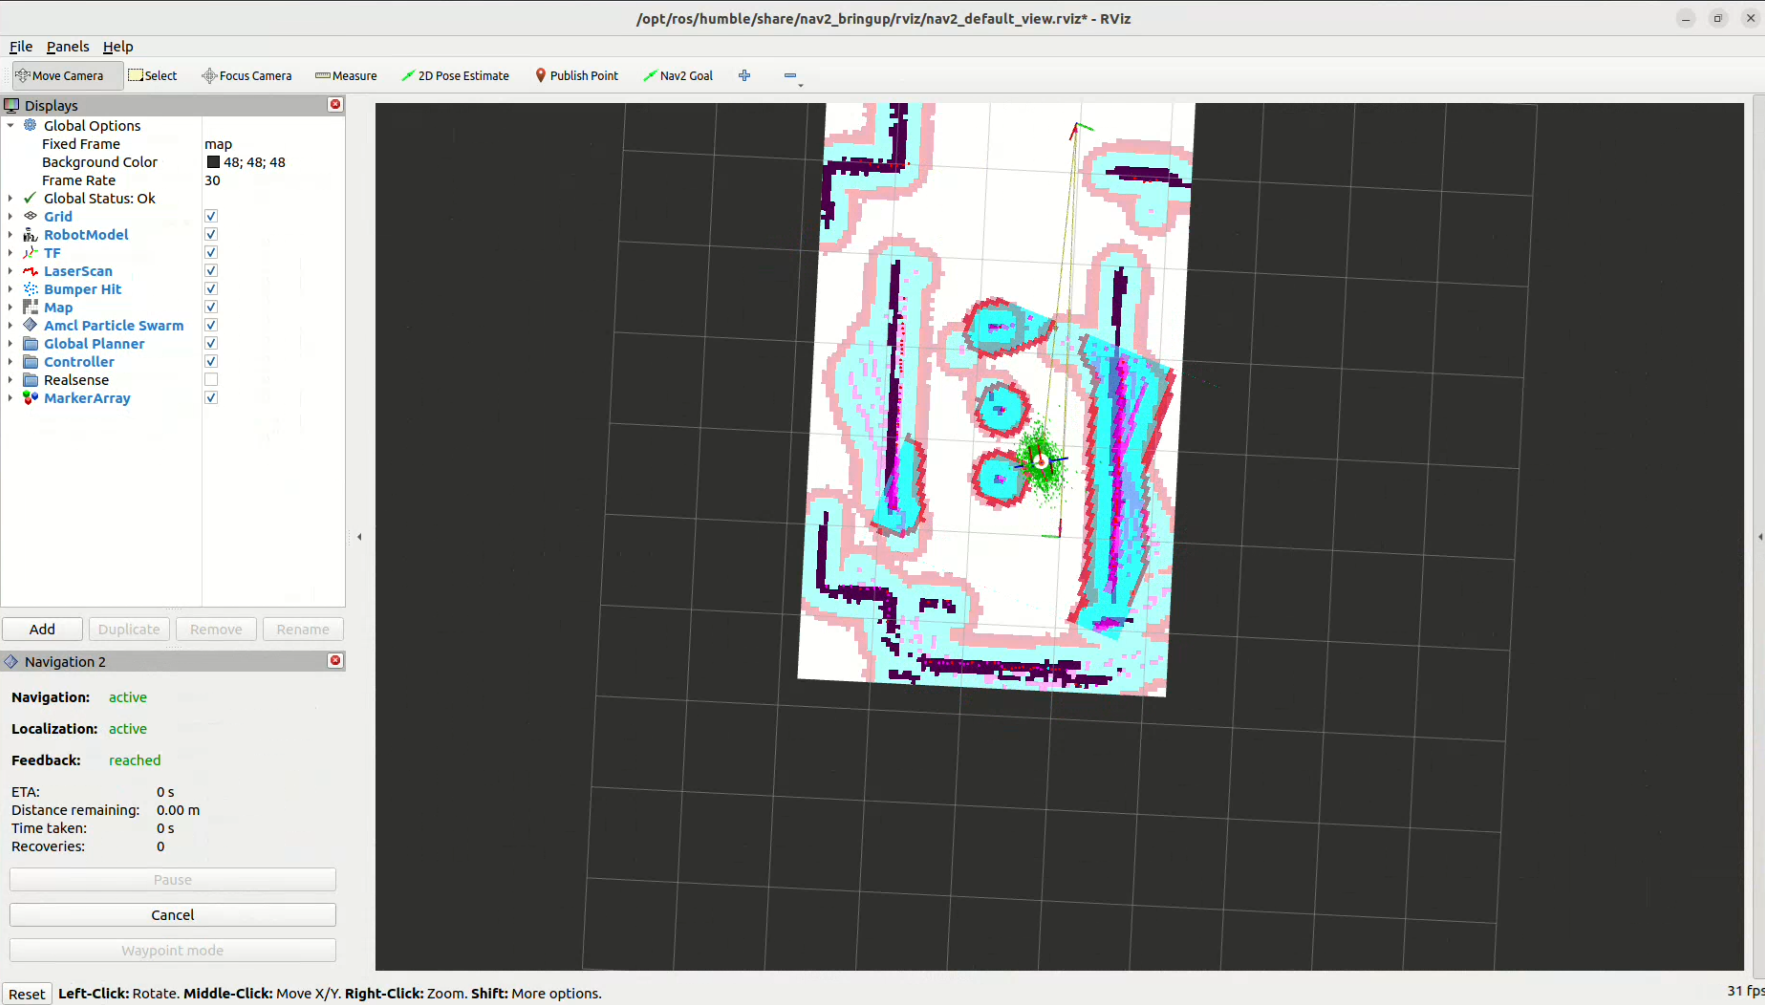
\includegraphics[width=1\textwidth]{images/launch-nav6.png}
	\caption{Dotarcie robota do celu.}
	\label{fig:nav-map6}
\end{figure}

\section{Administracja systemem}
System nie wymaga specjalnej administracji, jednakże w przypadku problemów z działaniem, można skorzystać z narzędzi diagnostycznych dostępnych w ROS 2, jak i z dokumentacji dostępnej na stronie internetowej ROS 2. W celu modyfikacji np. prędkością poruszania robota, przy korzystaniu z klawiatury, można zmienić prędkość przez naciśnięcie q i w. Do modyfikacji prędkości podczas nawigacji, można zmienić prędkość w pliku konfiguracyjnym Nav2 (nav2\_params.yaml).
\section{Kwestie bezpieczeństwa}
Robot opracowany został z myślą o omijaniu przeszkód, nawet tych których nie było na wcześniej stworzonej mapie pozwalając na bezpieczne poruszanie się w przestrzeni.
Należy jednak pamiętać że robot ten nie został przygotowany do pracy w środowiskach bez równego podłoża, dlatego należy unikać przemieszczania się po nierównym terenie co może prowadzić do przewrócenia się robota.
\newpage
\section{Scenariusze korzystania z systemu}

Robot ten pozwala na mapowanie różnego rodzaju pomieszczeń, oraz na nawigację do wyznaczonych punktów, co pozwala na zastosowanie go w różnego rodzaju zastosowaniach, jak np. inspekcja pomieszczeń. Testy przeprowadzane były w małych pomieszczeniach nie przekraczających 40 m$^2$, jednakże robot ten jest w stanie mapować pomieszczenia nawet do 24 000 m$^2$ co wynika z dokumentacji Nav2 \cite{bib:abs-2003-00368}.
%%%%%%%%%%%%%%%%%%%%%
%% RYSUNEK Z PLIKU
%
%\begin{figure}
%\centering
%
\includegraphics[width=0.5\textwidth]{./politechnika_sl_logo_bw_pion_pl.pdf}
%\caption{Podpis rysunku zawsze pod rysunkiem.}
%\label{fig:etykieta-rysunku}
%\end{figure}
%Rys. \ref{fig:etykieta-rysunku} przestawia …
%%%%%%%%%%%%%%%%%%%%%
%
%%%%%%%%%%%%%%%%%%%%%
%% WIELE RYSUNKÓW 
%
%\begin{figure}
%\centering
%\begin{subfigure}{0.4\textwidth}
%    
\includegraphics[width=\textwidth]{./politechnika_sl_logo_bw_pion_pl.pdf}
%    \caption{Lewy górny rysunek.}
%    \label{fig:lewy-gorny}
%\end{subfigure}
%\hfill
%\begin{subfigure}{0.4\textwidth}
%    
\includegraphics[width=\textwidth]{./politechnika_sl_logo_bw_pion_pl.pdf}
%    \caption{Prawy górny rysunek.}
%    \label{fig:prawy-gorny}
%\end{subfigure}
%
%\begin{subfigure}{0.4\textwidth}
%    
\includegraphics[width=\textwidth]{./politechnika_sl_logo_bw_pion_pl.pdf}
%    \caption{Lewy dolny rysunek.}
%    \label{fig:lewy-dolny}
%\end{subfigure}
%\hfill
%\begin{subfigure}{0.4\textwidth}
%    
\includegraphics[width=\textwidth]{./politechnika_sl_logo_bw_pion_pl.pdf}
%    \caption{Prawy dolny rysunek.}
%    \label{fig:prawy-dolny}
%\end{subfigure}
%        
%\caption{Wspólny podpis kilku rysunków.}
%\label{fig:wiele-rysunkow}
%\end{figure}
%Rys. \ref{fig:wiele-rysunkow} przestawia wiele ważnych informacji, np. rys. \ref{fig:prawy-gorny} jest na prawo u góry.
%%%%%%%%%%%%%%%%%%%%%


%
%\begin{figure}
%\centering
%\begin{tikzpicture}
%\begin{axis}[
%    y tick label style={
%        /pgf/number format/.cd,
%            fixed,   % po zakomentowaniu os rzednych jest indeksowana wykladniczo
%            fixed zerofill, % 1.0 zamiast 1
%            precision=1,
%        /tikz/.cd
%    },
%    x tick label style={
%        /pgf/number format/.cd,
%            fixed,
%            fixed zerofill,
%            precision=2,
%        /tikz/.cd
%    }
%]
%\addplot [domain=0.0:0.1] {rnd};
%\end{axis} 
%\end{tikzpicture}
%\caption{Podpis rysunku po rysunkiem.}
%\label{fig:2}
%\end{figure}


% TODO
\chapter{Specyfikacja techniczna}
\label{ch:05}
Rozdział ten zawiera specyfikację techniczną systemu, w tym opis wykorzystanych technologii, architekturę systemu, 
strukturę systemu, opis działania algorytmów oraz diagramy UML wyjaśniające działanie poszczególnych programów.
\section{Wykorzystane technologie} 
Projekt wykorzystuje następujące technologie:
\begin{itemize}
	\item ROS 2 Humble - platforma do tworzenia oprogramowania dla robotów
	\item SLAM Toolbox - pakiet do mapowania otoczenia
	\item Nav2 - pakiet do nawigacji robota wraz z algorytmem AMCL do lokalizacji
	\item ROS2 Control - platforma do sterowania robotem
	\item DiffDrive Arduino - pakiet zapewniający interfejs między ROS2 Control a Arduino
	\item ROS arduino bridge - pakiet zapewniający oprogramowanie do sterowania silnikami i zbierania danych z enkoderów
\end{itemize}
\newpage
\section{Architektura systemu}
Sposób działania systemu oparty jest na współdziałających ze sobą programach, których sposób połączenia zaprezentowano na rysunku \ref{fig:diagram-programy}.

\begin{figure}[!hb]
	\centering
	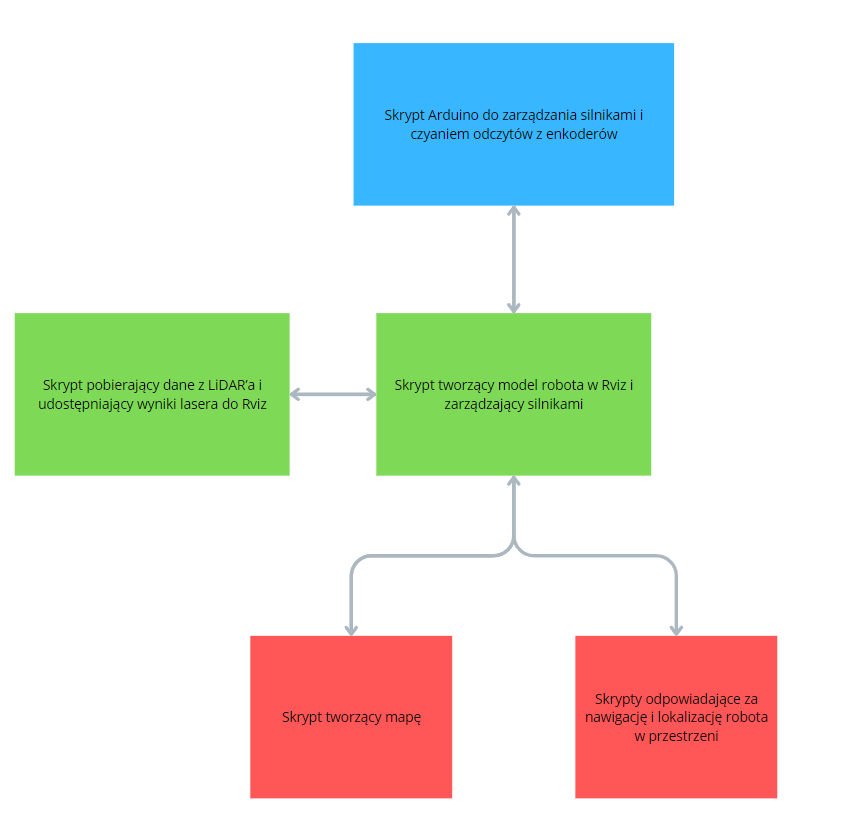
\includegraphics[width=1\textwidth]{images/diagram-programy.png}
	\caption{Wizualizacja połączenia skryptów w systemie}
	\label{fig:diagram-programy}
\end{figure}


\newpage
\section{Struktura systemu i objaśnienie działania algorytmów}

W tej sekcji zawarto szczegółowe opisy funkcjonalności każdego ze skryptów \ref{fig:diagram-programy}, które są odpowiedzialne za działanie robota.

Wszystkie skrypty znajdują się w załączniku Oprogramowanie.
\subsection{Arduino}
Oprogramowanie to odpowiedzialne jest za sterowanie silnikami i zbieranie danych z enkoderów. Opiera się na pakiecie ROS arduino bridge\cite{bib:rosarduinobridge}, który zapewnia interfejs między ROS 2 a Arduino. 


Program ten składa się z następujących plików:
\begin{itemize}
	\item ROSArduinoBridge.ino -  skrypt obsługuje komunikację szeregową z prędkością 57600 bodów (jednostka szybkości transmisji danych) i może kontrolować silniki poprzez różne sterowniki (np. Pololu VNH5019, MC33926 czy L298N). 
	Główna pętla programu ciągle nasłuchuje komend przychodzących przez port szeregowy, wykonuje obliczenia PID w regularnych odstępach czasu oraz aktualizuje stan serwomechanizmów jeśli są używane. Cały kod znajduje się w pliku ROSArduinoBridge.ino w załączniku Oprogramowanie.
	\newpage
	\item motor\_driver.ino - plik ten zawiera różne definicje sterowników silników, gdzie w tym projekcie wykorzystano  L298N, który jest dwukanałowym mostkiem H. Program obsługuje również inne sterowniki jak Pololu VNH5019 czy MC33926.

	W kodzie zaimplementowano trzy podstawowe funkcje:
	\begin{itemize}
	\item initMotorController() - inicjalizacja sterownika silników
	\item setMotorSpeed(int i, int spd) - ustawienie prędkości pojedynczego silnika 
	\item setMotorSpeeds(int leftSpeed, int rightSpeed) - funkcja do ustawiania prędkości obu silników
	\end{itemize}

	Dla sterownika L298N prędkość silników jest kontrolowana przez sygnały PWM wysyłane na odpowiednie piny. Ujemne wartości prędkości powodują obrót silnika w przeciwnym kierunku. Program zapewnia też ograniczenie maksymalnej prędkości do 255 (8-bit PWM).
	\item encoder\_driver.ino - Ten plik zawiera definicje obsługi enkoderów do odczytu pozycji kół robota. W implementacji wykorzystano przerwania do dokładnego zliczania impulsów z enkoderów.

	Plik zawiera między innymi:
	\begin{itemize}
	\item Definicje pinów dla enkoderów lewego i prawego koła
	\item Wykorzystanie przerwań PCINT (ang. "Pin Change Interrupt") do zliczania impulsów
	\item Funkcje do odczytu i resetowania liczników enkoderów
	\end{itemize}

	

	\begin{figure}[!hb]
		\centering
	\begin{lstlisting}
	/* Interrupt routine for LEFT encoder */
	ISR (PCINT2_vect){
		static uint8_t enc_last=0;	
		enc_last <<=2; //shift previous state
		enc_last |= (PIND & (3 << 2)) >> 2; //read current state
		left_enc_pos += ENC_STATES[(enc_last & 0x0f)];
	}
	/* Interrupt routine for RIGHT encoder */
	ISR (PCINT1_vect){
		static uint8_t enc_last=0;
		enc_last <<=2; //shift previous state
		enc_last |= (PINC & (3 << 4)) >> 4; //read current state
		right_enc_pos += ENC_STATES[(enc_last & 0x0f)];
	}
	\end{lstlisting}
	\caption{Fragment kodu źródłowego z pliku encoder\_driver.ino z obsługą przerwań do precyzyjnego zliczania impulsów z enkoderów}
	\label{fig:encoder-driver2}
	\end{figure}
\newpage
	\item encoder\_driver.h, oraz motor\_driver.h - pliki zawierające deklaracje funkcji i zmiennych, definiując porty i piny dla enkoderów i sterowników silników. 
	\newline

	
	\begin{figure}[!hb]
		\centering
	\begin{lstlisting}
		/*************************************************
		Motor driver function definitions - by James Nugen
		*************************************************/
	 
	 #ifdef L298_MOTOR_DRIVER
	   #define RIGHT_MOTOR_BACKWARD 5
	   #define LEFT_MOTOR_BACKWARD  6
	   #define RIGHT_MOTOR_FORWARD  9
	   #define LEFT_MOTOR_FORWARD   10
	   #define RIGHT_MOTOR_ENABLE 12
	   #define LEFT_MOTOR_ENABLE 13
	 #endif
	 
	 void initMotorController();
	 void setMotorSpeed(int i, int spd);
	 void setMotorSpeeds(int leftSpeed, int rightSpeed);
	 
		\end{lstlisting}
		\caption{Kod źródłowy z pliku motor\_driver.h}
		\label{fig:motor-driver}
		\end{figure}

	

	\begin{figure}[!hb]
		\begin{lstlisting}
			/* *************************************************************
			Encoder driver function definitions - by James Nugen
			************************************************************ */
			
			
		 #ifdef ARDUINO_ENC_COUNTER
		   //below can be changed, but should be PORTD pins; 
		   //otherwise additional changes in the code are required
		   #define LEFT_ENC_PIN_A PD2  //pin 2
		   #define LEFT_ENC_PIN_B PD3  //pin 3
		   
		   //below can be changed, but should be PORTC pins
		   #define RIGHT_ENC_PIN_A PC4  //pin A4
		   #define RIGHT_ENC_PIN_B PC5   //pin A5
		 #endif
			
		 long readEncoder(int i);
		 void resetEncoder(int i);
		 void resetEncoders();
			\end{lstlisting}
			\caption{Kod źródłowy z pliku encoder\_driver.h}
			\label{fig:encoder-driver}
			\end{figure}
			
			\item commands.h - zawiera definicje komend wysyłanych z Raspberry Pi do Arduino. W pliku zdefiniowano między innymi komendy do sterowania silnikami, odczytu enkoderów i resetowania enkoderów.
			\item diff\_controller.h - plik zawierający implementację regulatora PID dla sterowania prędkością kół robota. Regulator wykorzystuje zaawansowane techniki sterowania, w tym:

			\begin{itemize}
				\item Unikanie skoku pochodnej (ang. "derivative kick") poprzez wykorzystanie poprzedniego wejścia zamiast poprzedniego błędu
				\item Płynne dostrajanie parametrów dzięki użyciu członu całkującego ITerm zamiast scałkowanego błędu
				\item Inicjalizację zapobiegającą skokom przy uruchomieniu
				\item Anti-windup poprzez ograniczenie wyjścia i zatrzymanie całkowania gdy wyjście jest nasycone
			\end{itemize}

			Regulator PID (ang. "Proportional-Integral-Derivative"), w którym zastosowane zostały domyślne wartości po testach i zadowalających wynikach.  Działa w następujący sposób:
			\begin{itemize}
				\item Człon proporcjonalny (P) - generuje sygnał sterujący proporcjonalny do uchybu
				\item Człon całkujący (I) - eliminuje błąd w stanie ustalonym poprzez całkowanie uchybu
				\item Człon różniczkujący (D) - poprawia odpowiedź przejściową poprzez przewidywanie zmian uchybu
			\end{itemize}

			Plik zawiera struktury danych i funkcje do:
			\begin{itemize}
				\item Przechowywania stanu regulatora dla każdego koła
				\item Resetowania stanu regulatorów
				\item Obliczania nowych wartości sterujących
				\item Aktualizacji regulatorów na podstawie odczytów z enkoderów
			\end{itemize}
			
\end{itemize}
 
\newpage
\subsection{LiDAR}
Skrypt ten odpowiada za odczyt danych z LiDAR-a i przesyłanie ich do Raspberry Pi. Program ten wykorzystuje pakiet rplidar\_ros udostępniony przez producenta SLAMTEC. 
Do obsługi LiDAR-a stworzono plik wykonawczy rplidar.launch.py. Ten plik odpowiedzialny jest za konfigurację i uruchomienie węzła obsługującego czujnik RPLidar A1. 


Plik definiuje parametry pracy czujnika, takie jak:
\begin{itemize}
\item Port szeregowy do komunikacji z czujnikiem
\item Prędkość transmisji (115200 bodów)
\item Tryb skanowania (standardowy)
\item Częstotliwość publikowania danych (2,5 Hz)
\item Zakres pomiarowy (od 0,15 m do 12 m wynikający z parametrów czujnika)
\item Zakres kątowy skanowania (pełny obrót 360 stopni)
\end{itemize}

Program sprawdza również dostępność portu szeregowego i zgłasza odpowiedni komunikat w przypadku braku połączenia z czujnikiem. Dane z czujnika są publikowane do systemu ROS 2 i mogą być wykorzystywane przez inne węzły, na przykład do tworzenia mapy otoczenia czy nawigacji.

\subsection{Sterowanie silnikami i model robota}
Za sterowanie silnikami odpowiadają następujące pliki:
\begin{itemize}

	\item model\_controll.launch.py - główny plik wykonawczy sterujący robotem. Odpowiada za:
		\begin{itemize}
			\item Uruchomienie i konfigurację podstawowych komponentów sterowania:
			\begin{itemize}
				\item robot\_state\_publisher - publikuje transformacje robota na podstawie modelu URDF (ang. "Unified Robot Description Format")
				\item twist\_mux - zarządza priorytetyzacją komend prędkości, czyli przypisuje odpowiednie komendy do poprawnego korzystania z Ros2 Control i np. sterowania za pomocą klawiatury.
				\item controller\_manager - zarządza kontrolerami ROS2 Control
				\item diff\_cont - kontroler napędu różnicowego
				\item joint\_broad - nadawca stanu połączeń
			\end{itemize}
			\newpage
			\item Obsługę parametrów:
			\begin{itemize}
				\item use\_sim\_time (domyślnie: fałszywe) - przełącznik trybu symulacji
				\item use\_ros2\_control (domyślnie: prawdziwe) - włączanie/wyłączanie ROS2 Control
			\end{itemize}
			\item Sekwencyjne uruchamianie komponentów z opóźnieniami
			\item Ładowanie plików konfiguracyjnych (URDF, YAML)
		\end{itemize}

	\item model\_main.xacro - plik definiujący model kinematyczny i wizualny robota w formacie URDF/XACRO. Zawiera:
		\begin{itemize}
			\item Definicje materiałów do wizualizacji (biały - walec stanowiący korpus robota, pomarańczowy - LiDAR, niebieski - koła, czarny - koła podporowe)
			\item Strukturę robota:
			\begin{itemize}
				\item base\_link - podstawowy punkt odniesienia
				\item container - główny korpus w kształcie walca
				\item LiDAR - czujnik laserowy na górze konstrukcji
				\item Koła napędowe (lewe i prawe) - połączenia ciągłe (ang. "continuous joints"), zależne od prędkości (ang. "velocity dependent")
				\item Koła podporowe (przód i tył) - połączenia stałe (fixed joints)
			\end{itemize}
			\item Właściwości fizyczne elementów:
			\begin{itemize}
				\item Masy
				\item Momenty bezwładności
				\item Parametry kolizji
			\end{itemize}
		\end{itemize}
		Model ten umożliwia wizualizację robota w RVIZ oraz symulację jego dynamiki w środowisku ROS.
\newpage
	
	\item model.urdf.xacro - Jest to plik spajający definicję modelu z pliku model\_main.xacro z konfiguracją kontrolerów z pliku ros2\_control.xacro.
	
	\begin{figure}[!hb]
		\centering
	\begin{lstlisting}
		<?xml version="1.0"?>
		<robot xmlns:xacro="http://www.ros.org/wiki/xacro" name="robot_slam">
			<xacro:arg name="use_ros2_control" default="true"/>
			<xacro:arg name="sim_mode" default="false"/>
			<xacro:include filename="model_main.xacro"/>
			<xacro:include filename="ros2_control.xacro"/>
			<xacro:ros2_control_robot use_ros2_control="$(arg use_ros2_control)" sim_mode="$(arg sim_mode)"/>
		</robot>
		\end{lstlisting}
		\caption{Kod źródłowy pliku model.urdf.xacro}
		\label{fig:model.urdf.xacro}
	\end{figure}
	\item internal\_macros.xacro - plik zawiera momenty bezwładności dla poszczególnych elementów robota.

	\item ros2\_control.xacro - w tym pliku zawarto konfigurację silników dla Ros2 Control, zdefiniowano w nim nazwy dla poszczególnych kół, częstotliwość odświeżania zgodną z skryptem ROSArduinoBridge, czyli 57600 bodów, zliczenia enkoderów na obrót koła - 2194 wyznaczone przez testy, oraz ustawienie maksymalnej i minimalnej prędkości dla każdego silnika.
	\item twist\_mux.yaml - plik konfiguracyjny, wykorzystywany do udostępnienia cmd\_vel do sterowania robotem. Jest to potrzebne przy sterowaniu z klawiatury.
	\newpage \item my\_controllers.yaml - jest to plik konfiguracyjny potrzebny do integracji systemu z pakietem diffdrive arduino. Zdefiniowano w nim nazwy kół zgodne z poprzednimi plikami konfiguracyjnymi, częstotliwość aktualizacji, szerokość kół i ich rozstaw.
	\begin{figure}[!hb]
		\centering
	\begin{lstlisting}
		ros__parameters:

		publish_rate: 50.0  # Increased for better velocity updates
	
		base_frame_id: base_footprint  # Reverted frame
	
		left_wheel_names: ['left_wheel_joint']
		right_wheel_names: ['right_wheel_joint']
		wheel_separation: 0.14  
		wheel_radius: 0.035     
	
		use_stamped_vel: false
	
		\end{lstlisting}
		\caption{Fragment kodu z pliku my\_controllers.yaml}
		\label{fig:my-controllers}
	\end{figure}
\end{itemize}
\newpage
\subsection{Mapowanie}
W celu mapowania otoczenia robota wykorzystano pakiet SLAM Toolbox, który pozwala na tworzenie mapy otoczenia na podstawie danych z LiDAR-a. Utworzony program składa się z następujących plików:
\begin{itemize}
	\item slam.launch.py - plik ten odpowiada za konfigurację i uruchomienie węzła odpowiedzialnego za mapowanie otoczenia. 
	Program ten publikuje mapę otoczenia w systemie ROS 2, która może być wykorzystywana do nawigacji robota.
	\item mapper\_params\_online\_async.yaml - plik konfiguracyjny zawarty w pakiecie SLAM Toolbox, wybrana została wersja online async, zamiast online sync, ze względu na lepszą wydajność. W pliku zdefiniowano parametry pracy algorytmu, takie jak:
	
	\begin{figure}[!hb]
		\centering
	\begin{lstlisting}
    solver_plugin: solver_plugins::CeresSolver
    ceres_linear_solver: SPARSE_NORMAL_CHOLESKY
    ceres_preconditioner: SCHUR_JACOBI
    ceres_trust_strategy: LEVENBERG_MARQUARDT
    ceres_dogleg_type: TRADITIONAL_DOGLEG
    ceres_loss_function: HUBERLOSS  # Changed from None
    ceres_huber_loss_delta: 2.0  
\end{lstlisting}
\caption{Fragment kodu z pliku mapper\_params\_online\_async.yaml}
\label{fig:mapper-params1}
\end{figure}
Wprowadzono tutaj zmianę w funkcji straty z None na HuberLoss, co pozwala na lepsze radzenie sobie z błędami wynikającymi z ślizgania się kół robota.

Kluczowym elementem jaki należy tutaj opisać jest wykorzystanie biblioteki Ceres Solver \cite{bib:Agarwal_Ceres_Solver_2022}. Jest to narzędzie, które pomaga znaleźć najlepsze dopasowanie między różnymi pomiarami, minimalizując błąd średniokwadratowy. Dzięki temu SLAM Toolbox może tworzyć dokładne mapy, nawet gdy niektóre pomiary są niedokładne lub błędne. 
\newline
Działa to na zasadzie iteracyjnego poprawiania oszacowań pozycji robota:

\begin{equation}
\min_x \frac{1}{2}\sum_{i} \rho_i(\|f_i(x_i)\|^2)
\end{equation}


\begin{itemize}
\item $x$ to pozycje robota, które chcemy znaleźć 
\item $f_i(x_i)$ mierzy, jak bardzo nasze oszacowanie pozycji różni się od rzeczywistych pomiarów
\item $\rho_i$ to funkcja, która pomaga ignorować błędne pomiary (działa jako filtr odrzucający "podejrzane" dane)
\item Cały proces dąży do znalezienia takich pozycji robota, dla których suma wszystkich błędów jest najmniejsza
\end{itemize}

Algorytm działa iteracyjnie, wykorzystuje do tego metodę Levenberga-Marquardta, która łączy w sobie:

\begin{itemize}
\item Szybkość metody Gaussa-Newtona (dobre do precyzyjnych korekt)
\item Stabilność metody największego spadku (pomocne przy większych korektach)
\end{itemize}

Dzięki takiemu podejściu SLAM Toolbox może tworzyć dokładne mapy, nawet gdy niektóre pomiary są niedokładne.

\begin{figure}[!hb]
	\centering
\begin{lstlisting}
	# ROS Parameters
    odom_frame: "odom"
    map_frame: "map"
    base_frame: "base_footprint"
    scan_topic: "/scan"
    use_map_saver: true
    use_sim_time: false
    mode: "mapping" #localization
\end{lstlisting}
\caption{Fragment kodu z pliku mapper\_params\_online\_async.yaml}
\label{fig:mapper-params2}
\end{figure}
Ustawiono tutaj tryb mapowania, oraz nazwy ramek, z których korzysta program.
\newline
\newpage
\begin{figure}[!hb]
	\centering
\begin{lstlisting}
	debug_logging: false
    throttle_scans: 2
    transform_publish_period: 0.05 #if 0 never publishes odometry
    map_update_interval: 2.0
    resolution: 0.05
    max_laser_range: 12.0 #RP Lidar A1
    minimum_time_interval: 0.2
    transform_timeout: 0.5
    tf_buffer_duration: 30.
    stack_size_to_use: 60000000 #// program needs a larger stack size
    enable_interactive_mode: true
\end{lstlisting}
\caption{Fragment kodu z pliku mapper\_params\_online\_async.yaml}
\label{fig:mapper-params3}
\end{figure}
Dostosowano parametry po przeprowadzeniu testów i analizie wyników. Zmniejszono odstęp czasowy między aktualizacjami mapy, zwiększono rozdzielczość mapy oraz zwiększono czas oczekiwania na transformację. Dostosowano również rozmiar stosu, aby zapobiec przepełnieniu pamięci. Zmieniony został też maksymalny dystans na jaki pozwala zamontowany model LiDAR-a.
\end{itemize}
\newpage
\subsection{Nawigacja i lokalizacja}
Do nawigacji i lokalizacji robota wykorzystano pakiet Nav2, który pozwala na wyznaczanie trasy i lokalizację robota na mapie. Program ten składa się z następujących plików:
\begin{itemize}
	\item nav\_localization.launch.py - plik ten odpowiada za konfigurację i uruchomienie węzłów odpowiedzialnych za nawigację i lokalizację robota. 
	 Podstawowym elementem jest serwer mapy, który przechowuje i udostępnia mapę otoczenia. Za lokalizację odpowiada algorytm AMCL (adaptacyjna lokalizacja Monte Carlo), który wykorzystuje chmurę cząstek do określenia pozycji robota na mapie. System kontroli ruchu składa się z kontrolera ruchu, który steruje silnikami, planera ścieżki wyznaczającego trasę oraz modułu zachowań awaryjnych, który pozwala na reagowanie w sytuacjach nieoczekiwanych. Całością zarządza nawigator oparty na drzewach zachowań.

	Program konfiguruje się poprzez zestaw parametrów, z których najważniejsze to praca w czasie rzeczywistym (zamiast symulacji), automatyczne uruchomienie systemu oraz ścieżki do plików z mapą i konfiguracją. 

	Szczególną uwagę poświęcono konfiguracji modułu AMCL, gdzie określono liczbę wykorzystywanych cząstek (od 3000 do 10000), parametry modelu ruchu (wszystkie ustawione na 0.2) oraz warunki aktualizacji lokalizacji (minimalny przesuw 0.1m i obrót 0.1 radiana). Dodatkowo włączono funkcję globalnej lokalizacji przy starcie systemu, co pozwala na określenie pozycji bez znajomości stanu początkowego.

	Do nawigacji tworzone są dodatkowe mapy kosztów (ang. "costmap") lokalna i globalna. Lokalna mapa kosztów odpowiada za omijanie obiektów które nie były na mapie podczas jej tworzenia, natomiast globalna mapa kosztów tworzy strefy wokół obiektów już zmapowanych, czyli np. ściany, co pozwala na tworzenie tras wokół przeszkód.
	\newpage
	\item amcl.yaml - plik konfiguracyjny algorytmu AMCL odpowiedzialnego 
	za precyzyjną lokalizację robota na mapie. Zawiera parametry takie jak:
	\begin{itemize}
		\item Współczynniki szumu odometrii (alpha1-5) ustawione na 0.2 dla zoptymalizowanej dokładności
		\item Parametry filtracji wiązki lasera dla lepszej jakości skanów
		\item Liczba cząstek (500-3000) dobrana dla optymalnej równowagi między dokładnością a wydajnością
		\item Częstotliwość aktualizacji pozycji i orientacji (co 0.1m/rad) zapewniająca płynne śledzenie
		\item Parametry adaptacji (szybkiej i wolnej) dla stabilnej lokalizacji
		\item Konfiguracja ramek odniesienia i transformacji dla poprawnej integracji z systemem ROS
	\end{itemize}
	\end{itemize}
\newpage
\section{Diagramy UML prezentujące działanie konkretnych programów}
\begin{figure}[!hb]
	\centering
	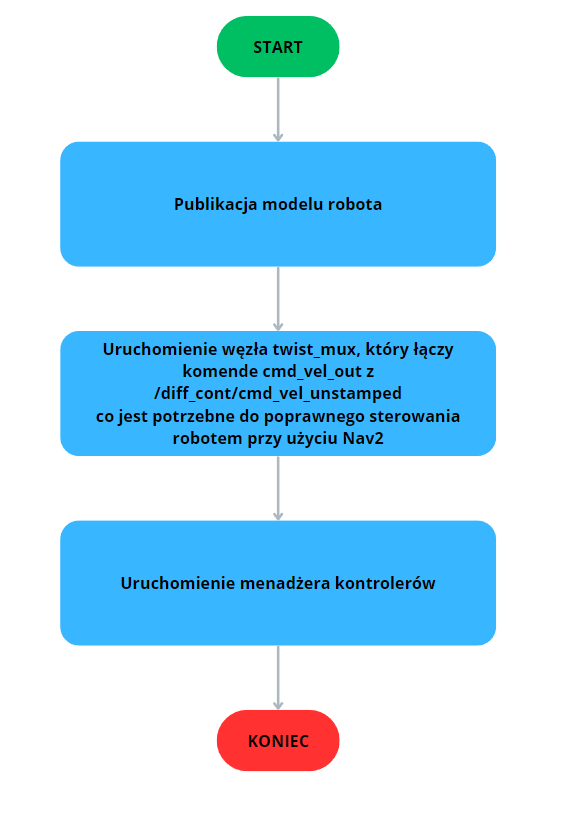
\includegraphics[width=0.8\textwidth]{images/uml-model.png}
	\caption{Diagram UML prezentujący działanie programu model\_controll.launch.py}
	\label{fig:diagram-model}
\end{figure}

\begin{figure}[!hb]
	\centering
	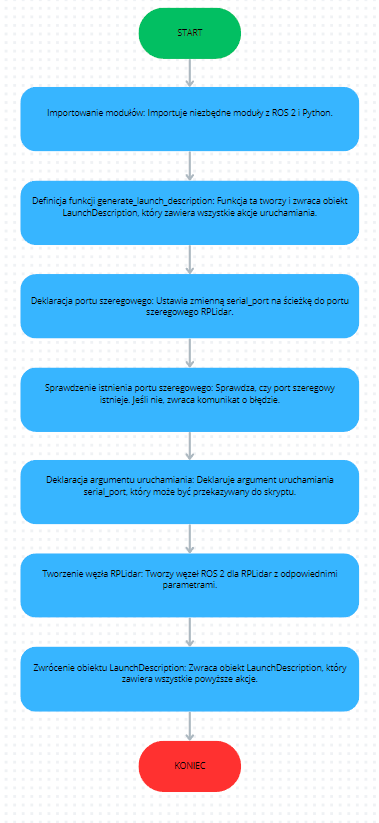
\includegraphics[width=0.9\textwidth]{images/uml-lidar.png}
	\caption{Diagram UML prezenujący działanie programu rplidar.launch.py}
	\label{fig:diagram-lidar}
\end{figure}

\begin{figure}[!hb]
	\centering
	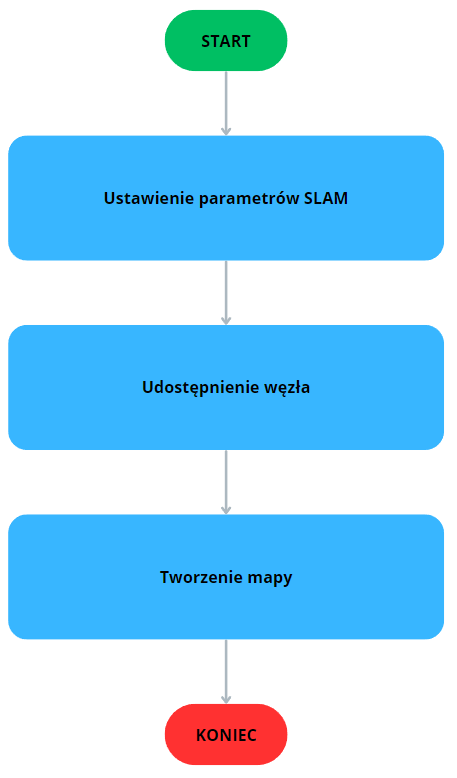
\includegraphics[width=0.9\textwidth]{images/uml-local.png}
	\caption{Diagram UML prezenujący działanie programu slam.launch.py}
	\label{fig:diagram-loc}
\end{figure}
\begin{figure}[!hb]
	\centering
	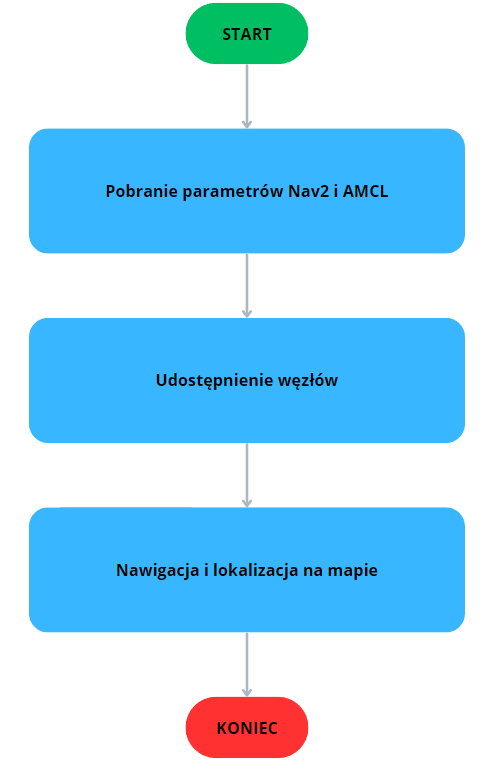
\includegraphics[width=0.9\textwidth]{images/uml-nav.png}
	\caption{Diagram UML prezenujący działanie programu nav\_localization.launch.py}
	\label{fig:diagram-nav}
\end{figure}


% % % % % % % % % % % % % % % % % % % % % % % % % % % % % % % % % % % 
% Pakiet minted wymaga importu: \usepackage{minted}                 %
% i specjalnego kompilowania:                                       %
% pdflatex -shell-escape main                                       %
% % % % % % % % % % % % % % % % % % % % % % % % % % % % % % % % % % % 


%Krótka wstawka kodu w linii tekstu jest możliwa, np.  \lstinline|int a;| (biblioteka \texttt{listings})% lub  \mintinline{C++}|int a;| (biblioteka \texttt{minted})
 
%Dłuższe fragmenty lepiej jest umieszczać jako rysunek, np. kod na rys \ref{fig:pseudokod:listings}% i rys. \ref{fig:pseudokod:minted}
%, a naprawdę długie fragmenty – w załączniku.


%\begin{figure}
%\centering
%\begin{lstlisting}
%class test : public basic
%{
%    public:
%      test (int a);
%      friend std::ostream operator<<(std::ostream & s, 
%                                     const test & t);
%    protected:
%      int _a;  
%      
%};
%\end{lstlisting}
%\caption{Pseudokod w \texttt{listings}.}
%\label{fig:pseudokod:listings}
%\end{figure}

%\begin{figure}
%\centering
%\begin{minted}[linenos,frame=lines]{c++}
%class test : public basic
%{
%    public:
%      test (int a);
%      friend std::ostream operator<<(std::ostream & s, 
%                                     const test & t);
%    protected:
%      int _a;  
%      
%};
%\end{minted}
%\caption{Pseudokod w \texttt{minted}.}
%\label{fig:pseudokod:minted}
%\end{figure}




% TODO
\chapter{Weryfikacja i walidacja}
W ramach pracy zastosowano model V do testowania systemu. Jest on popularnym modelem w inżynierii oprogramowania, który przedstawia proces tworzenia oprogramowania w formie litery V. Jej lewa strona reprezentuje fazy definiowania wymagań i projektowania systemu, natomiast prawa strona reprezentuje fazy testowania i walidacji systemu. 
\begin{figure}[!hb]
	\centering
	\includegraphics[width=1\textwidth]{images/modelV.png}
	\caption{Model V}
	\label{fig:modelv}
\end{figure}
\newpage
\section{Model V}

\begin{itemize}
	\item \textbf{Wymagania projektu:} Główne cele i założenia:
	\begin{itemize}
		\item Automatyczne tworzenie mapy otoczenia
		\item Autonomiczna nawigacja robota
		\item Precyzyjna lokalizacja
		\item Wykrywanie i omijanie przeszkód
	\end{itemize}

	\item \textbf{Analiza wymagań i tematu:} Szczegółowe wymagania funkcjonalne:
	\begin{itemize}
		\item Zdalne sterowanie robotem
		\item Zapisywanie i odczyt map
		\item Autonomiczna nawigacja do zadanych punktów
		\item Bezpieczne poruszanie się
	\end{itemize}

	\item \textbf{Architektura projektu:} Ogólna struktura systemu:
	\begin{itemize}
		\item Podział na podsystemy (napęd, sensory, sterowanie)
		\item Przepływ danych między modułami
		\item Interfejsy komunikacyjne
		\item Wybór technologii (ROS 2, Nav2, SLAM Toolbox)
	\end{itemize}

	\item \textbf{Architektura komponentów:} Projektowanie szczegółowe:
	\begin{itemize}
		\item Dobór komponentów sprzętowych
		\item Projekt mechaniczny i elektryczny
		\item Struktura oprogramowania
		\item Interfejsy programowe
	\end{itemize}

	\item \textbf{Implementacja:} Realizacja systemu:
	\begin{itemize}
		\item Budowa robota
		\item Programowanie sterowników
		\item Integracja sensorów
		\item Implementacja algorytmów
	\end{itemize}
\newpage
	\item \textbf{Testowanie komponentów:} Testy jednostkowe:
	\begin{itemize}
		\item Weryfikacja napędów
		\item Testy sensorów
		\item Sprawdzenie sterowników
		\item Testy algorytmów
	\end{itemize}

	\item \textbf{Testowanie interfejsów:} Testy integracyjne:
	\begin{itemize}
		\item Komunikacja między modułami
		\item Synchronizacja danych
		\item Przepływ informacji
		\item Współpraca komponentów
	\end{itemize}

	\item \textbf{Testowanie systemu:} Testy całościowe:
	\begin{itemize}
		\item Mapowanie otoczenia
		\item Lokalizacja robota
		\item Planowanie trasy
		\item Omijanie przeszkód
	\end{itemize}

	\item \textbf{Testy końcowe:} Walidacja systemu:
	\begin{itemize}
		\item Weryfikacja funkcjonalności
		\item Testy wydajności
		\item Testy niezawodności
		\item Zgodność z wymaganiami
	\end{itemize}
\end{itemize}
\newpage
\section{Organizacja eksperymentów}

\begin{itemize}
	\item \textbf{Testowanie jednostkowe:} Każdy moduł systemu, taki jak sterowanie silnikami, odczyt danych z LiDAR-a, tworzenie mapy, lokalizacja i nawigacja, został przetestowany indywidualnie. Testy jednostkowe obejmowały sprawdzenie poprawności działania poszczególnych funkcji i metod.
	\item \textbf{Testowanie integracyjne:} Po zakończeniu testów jednostkowych, moduły zostały zintegrowane i przetestowane pod kątem poprawności współdziałania. Testy integracyjne obejmowały sprawdzenie komunikacji między modułami oraz poprawności przesyłania danych, jak i ewentualnych błędów.
	\item \textbf{Testowanie systemowe:} Cały system został przetestowany w warunkach rzeczywistych. Testy systemowe obejmowały sprawdzenie poprawności działania systemu w różnych scenariuszach, takich jak zdalne sterowanie robotem, tworzenie mapy otoczenia, lokalizacja robota na mapie oraz autonomiczna nawigacja do wyznaczonych punktów.
	\item \textbf{Walidacja:} System został zweryfikowany pod kątem spełnienia wymagań użytkownika. Walidacja obejmowała sprawdzenie, czy system działa zgodnie z założeniami i spełnia oczekiwania użytkownika.
\end{itemize}

\section{Przypadki testowe}
Przypadki testowe obejmowały następujące scenariusze:
\begin{itemize}
	\item \textbf{Testowanie zdalnego sterowania:} Sprawdzenie, czy robot reaguje poprawnie na polecenia z klawiatury.
	\item \textbf{Testowanie tworzenia mapy:} Sprawdzenie, czy system poprawnie tworzy mapę otoczenia na podstawie danych z LiDAR-a.
	\item \textbf{Testowanie lokalizacji:} Sprawdzenie, czy system poprawnie lokalizuje robota na zapisanej mapie.
	\item \textbf{Testowanie nawigacji:} Sprawdzenie, czy system poprawnie planuje trasę i nawigację robota do wyznaczonych punktów, omijając przeszkody.
\end{itemize}
\newpage
\section{Wykryte i usunięte błędy}
Podczas testowania systemu wykryto i usunięto następujące błędy:
\begin{itemize}
	\item \textbf{Problem z zasilaniem:} Występowały problemy z zasilaniem Raspberry Pi, co zostało rozwiązane przez wyłączenie zbędnej funkcji szukania monitora. Rozwiązano ten problem przez zastosowanie komendy sudo systemctl set-default multi-user.target.
	\item \textbf{Problem z kołami:} Przez rozmiar kół i materiał z jakich zostały wykonane, robot miał problem z ślizganiem się kół co powodowało różnice między rzeczywistą pozycją robota, a tą która była wyznaczana podczas mapowania. Rozwiązano ten problem poprzez zastosowanie funkcji HuberLoss w algorytmie mapowania.
	\item \textbf{Problem z błędną lokalizacją robota na mapie:} Na wczesnym etapie testów pojawił się problem z sterowaniem robotem, który również uniemożliwiał nawgiację przy użyciu Nav2. Powodował sytuacje gdy podczas mapowania robot oddalał się od ściany w RVIZ zbliżał się do niej i po chwili model przenosił się na poprawne miejsce, powodowało to zmapowanie 2 ścian - poprawnej i przed przeniesieniem. Rozwiązaniem problemu było poprawne podłączenie silników do sterownika i Arduino.
\end{itemize}






% TODO
\chapter{Podsumowanie i wnioski}



\section{Uzyskane wyniki}
W wyniku przeprowadzonych prac udało się zrealizować wszystkie założone cele projektu. System autonomicznej nawigacji robota mobilnego został zaprojektowany, zaimplementowany i przetestowany. Robot poprawnie tworzy mapę otoczenia, lokalizuje się na zapisanej mapie oraz nawigował do wyznaczonych punktów, omijając przeszkody. 
\begin{figure}[!hb]
	\centering
	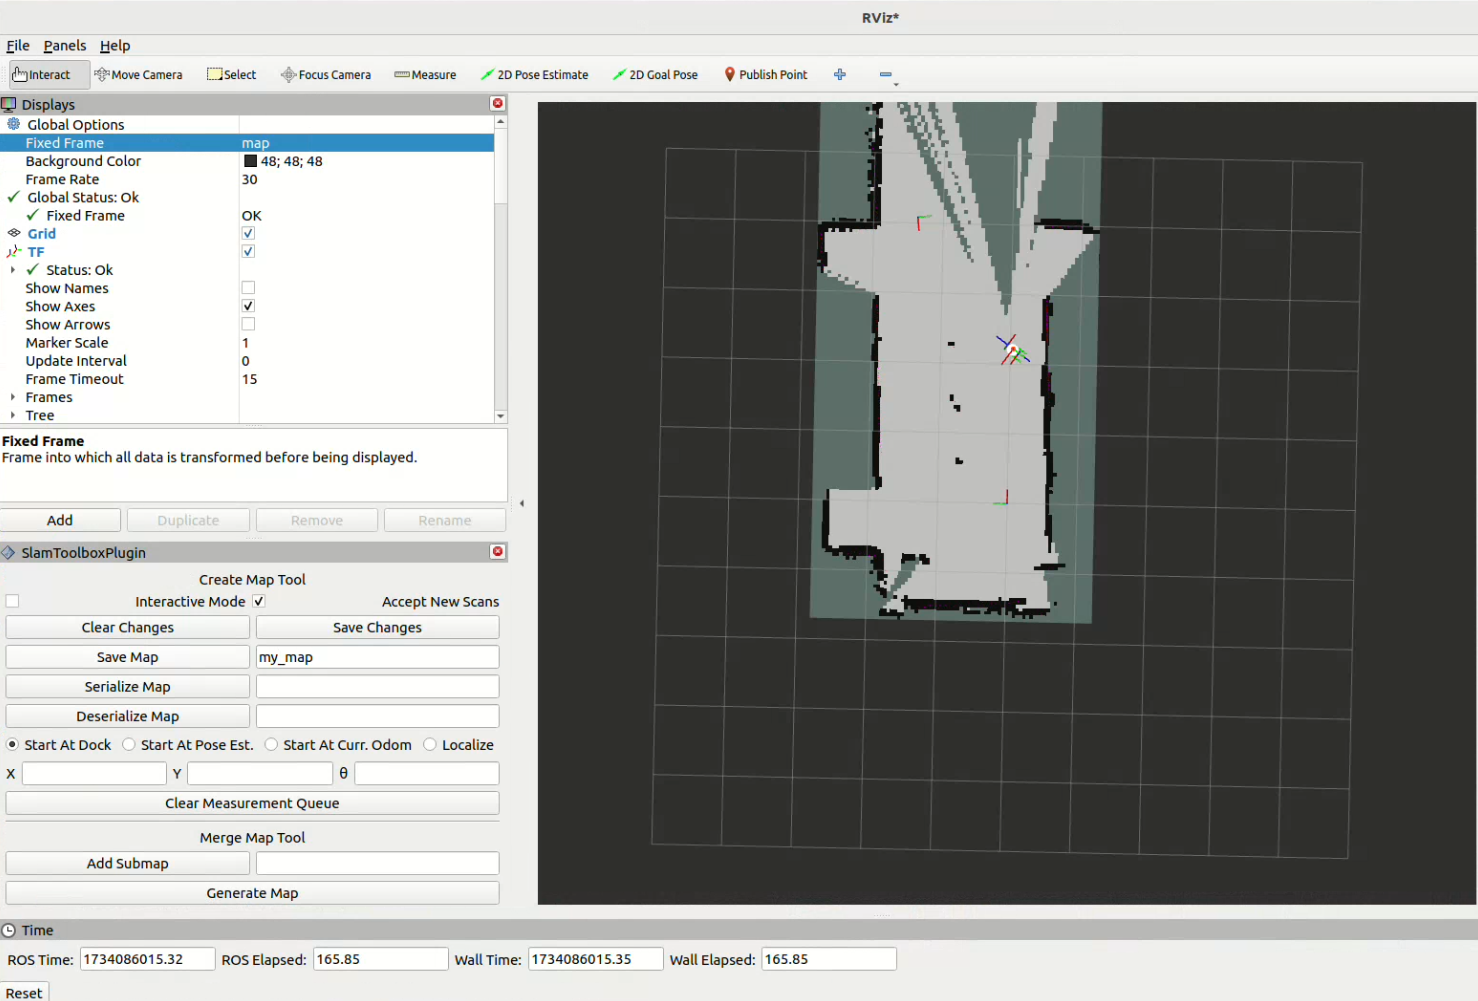
\includegraphics[width=1\textwidth]{images/save-map.png}
	\caption{Wizualizacja mapy otoczenia.}
	\label{fig:save-map2}
\end{figure}
\newpage
\begin{figure}[!hb]
	\centering
	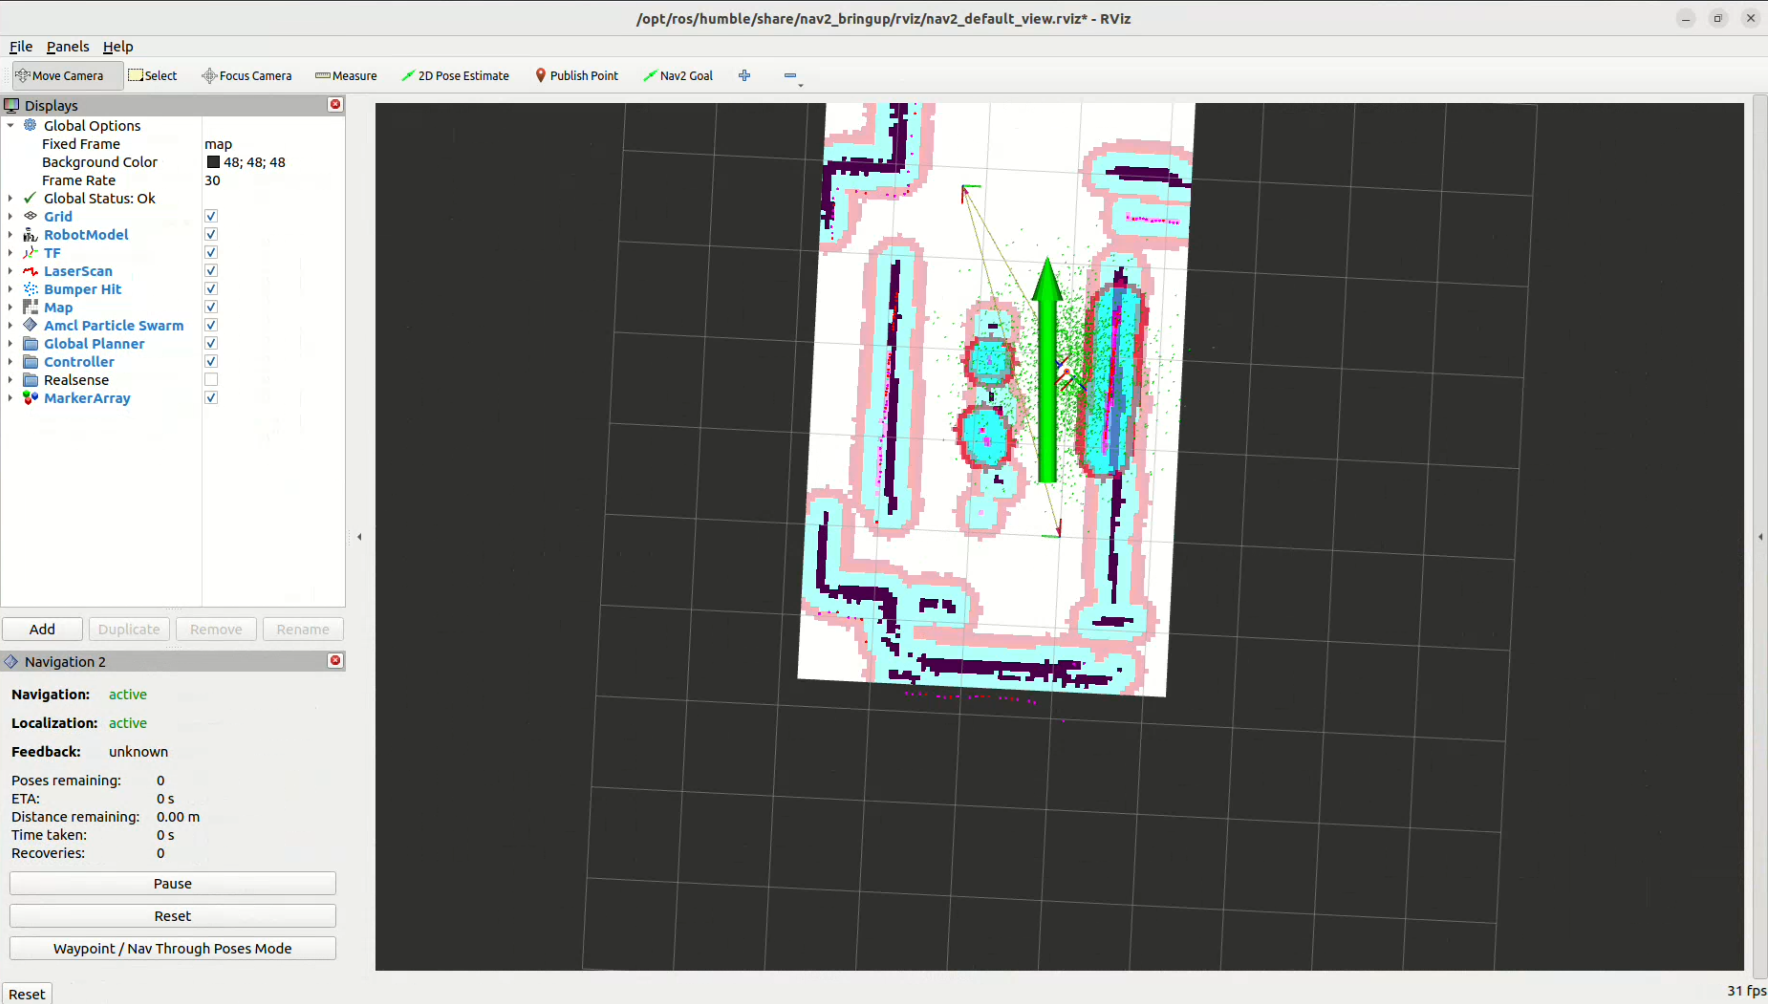
\includegraphics[width=1\textwidth]{images/launch-nav3.png}
	\caption{Rozpoczęcie nawigacji.}
	\label{fig:nav-map34}
\end{figure}

\begin{figure}[!hb]
	\centering
	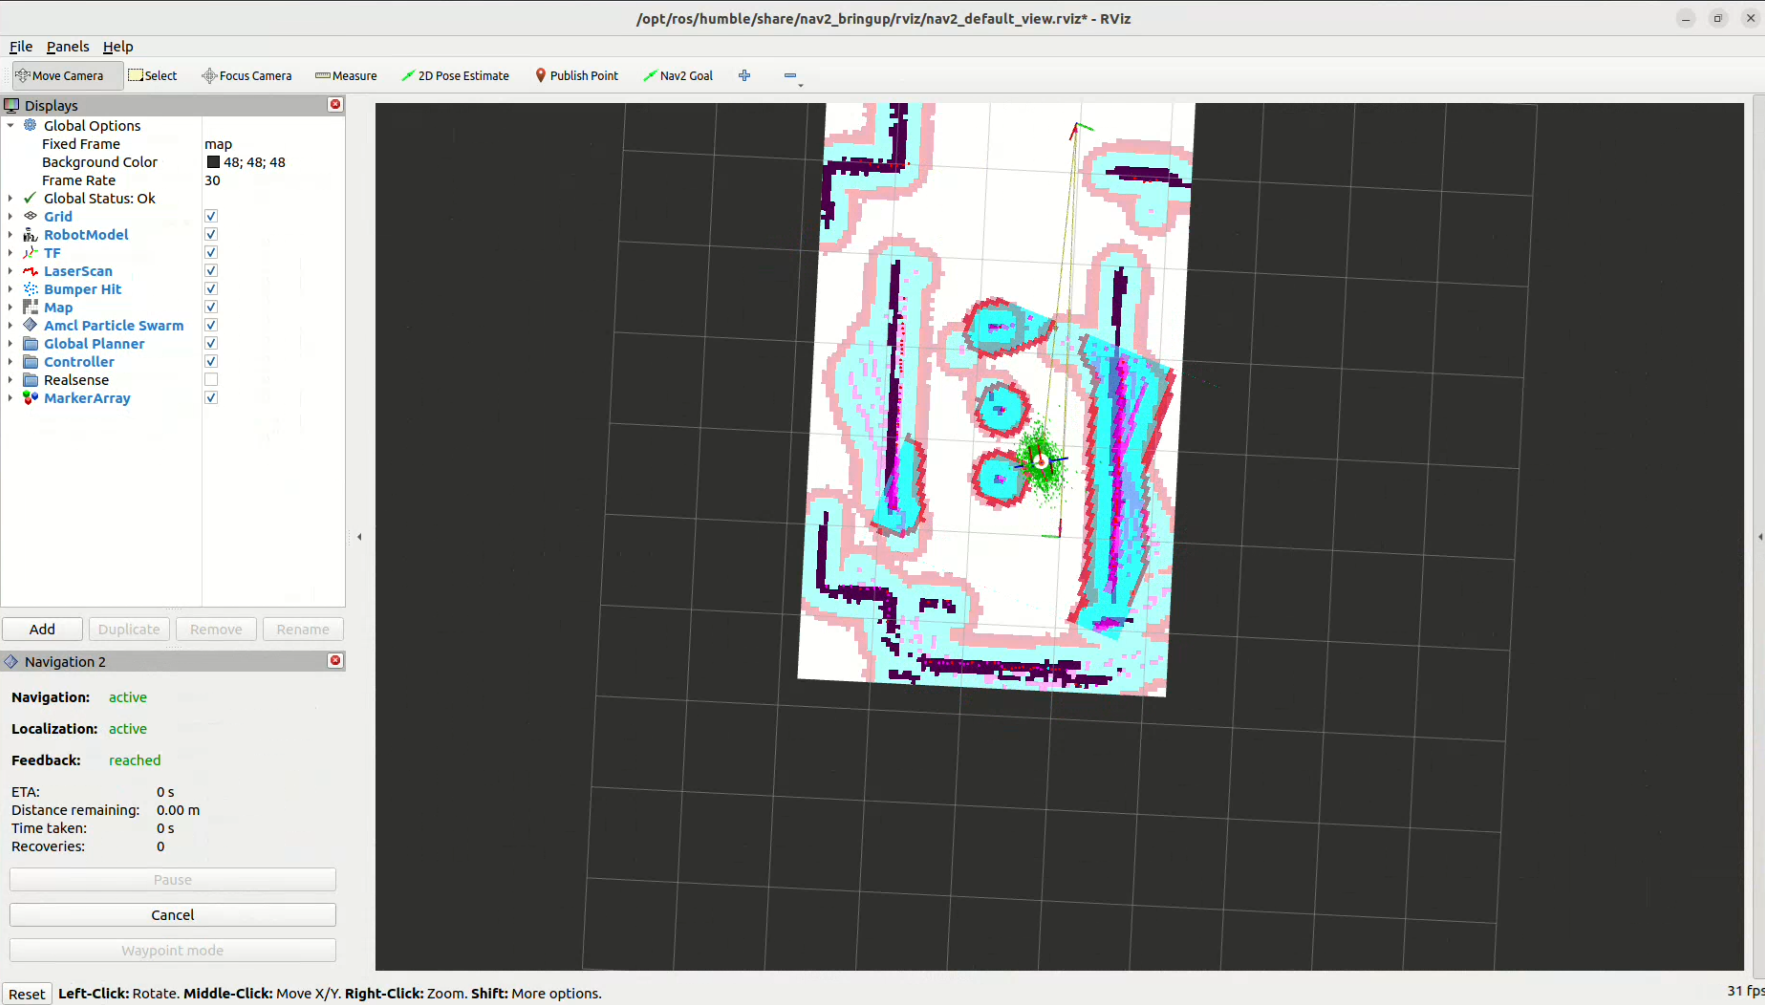
\includegraphics[width=1\textwidth]{images/launch-nav6.png}
	\caption{Dotarcie do celu}
	\label{fig:nav-map345}
\end{figure}
\newpage
\section{Kierunki dalszych prac}
W przyszłości możliwe jest rozszerzenie funkcjonalności systemu o dodatkowe elementy, takie jak:
\begin{itemize}
	\item Integracja z dodatkowymi sensorami, takimi jak kamery RGB-D, aby poprawić dokładność mapowania i lokalizacji.
	\item Rozbudowa systemu o możliwość ładowania akumulatorów bez potrzeby wyciągania ich z robota i zamontowanie modułu BMS.
	\item Stworzenie obudowy dla robota, aby zabezpieczyć go przed uszkodzeniami mechanicznymi.
\end{itemize}



\backmatter

%\bibliographystyle{plplain}  % bibtex
%\bibliography{biblio} % bibtex
\addcontentsline{toc}{chapter}{Bibliografia}
\printbibliography
\begin{appendices}

% TODO
\chapter{Spis skrótów i symboli}

\begin{itemize}
\item[SLAM] jednoczesna lokalizacja i mapowanie (ang. \english{Simultaneous Localization and Mapping})
\item[LiDAR] urządzenie wykonujące wykrywanie światła i określanie odległości (ang. \english{Light Detection and Ranging})
\item[IMU] inercyjna jednostka pomiarowa (ang. \english{Inertial Measurement Unit})
\item[RGB-D] kamera rejestrująca obraz RGB oraz informację o głębi (ang. \english{RGB-Depth})
\item[Nav2] system nawigacji dla ROS 2 (ang. \english{Navigation 2})
\item[ROS] system operacyjny dla robotów (ang. \english{Robot Operating System})
\item[ROS2 Control] system kontroli robotów dla ROS 2 (ang. \english{Robot Operating System 2 Control})
\item[SLAM Toolbox] zestaw narzędzi do jednoczesnej lokalizacji i mapowania (ang. \english{Simultaneous Localization and Mapping Toolbox})
\end{itemize}


% TODO
%\chapter{Źródła}

%Jeżeli w pracy konieczne jest umieszczenie długich fragmentów kodu źródłowego, należy je przenieść w to miejsce.

%\begin{lstlisting}
%if (_nClusters < 1)
%	throw std::string ("unknown number of clusters");
%if (_nIterations < 1 and _epsilon < 0)
%	throw std::string ("You should set a maximal number of iteration or minimal difference -- epsilon.");
%if (_nIterations > 0 and _epsilon > 0)
%	throw std::string ("Both number of iterations and minimal epsilon set -- you should set either number of iterations or minimal epsilon.");
%\end{lstlisting}


% % % % % % % % % % % % % % % % % % % % % % % % % % % % % % % % % % % 
% Pakiet minted wymaga odkomentowania w pliku config/settings.tex   %
% importu pakietu minted: \usepackage{minted}                       %
% i specjalnego kompilowania:                                       %
% pdflatex -shell-escape praca                                      %
% % % % % % % % % % % % % % % % % % % % % % % % % % % % % % % % % % % 

%\begin{minted}[linenos,breaklines,frame=lines]{c++}
%if (_nClusters < 1)
%   throw std::string ("unknown number of clusters");
%if (_nIterations < 1 and _epsilon < 0)
%   throw std::string ("You should set a maximal number of iteration or minimal difference -- epsilon.");
%if (_nIterations > 0 and _epsilon > 0)
%   throw std::string ("Both number of iterations and minimal epsilon set -- you should set either number of iterations or minimal epsilon.");
%\end{minted}


% TODO
\chapter{Lista dodatkowych plików, uzupełniających tekst pracy} 

Do pracy załączono następujące dodatkowe pliki:
\begin{itemize}
	\item Pliki źródłowe programu w folderze \texttt{Oprogramowanie}
	\item Film pokazujący działanie robota w pliku \texttt{Robot.mp4}
	\end{itemize}



\listoffigures
\addcontentsline{toc}{chapter}{Spis rysunków}
%\listoftables
%\addcontentsline{toc}{chapter}{Spis tabel}

\end{appendices}

\end{document}


%% Finis coronat opus.

